\section{Implementaci\'on existente}
Antes de describir las mejoras realizadas sobre la aplicaci\'on existente, vamos a ver
los pasos que componen la construcci\'on de la matriz de Kohn-Sham, necesario para el
c\'alculo de las fuerzas \'inter at\'omicas de QM, representadas en la funci\'on de onda y
la energ\'ia del sistema.

\begin{figure}[htbp]
   \centering
   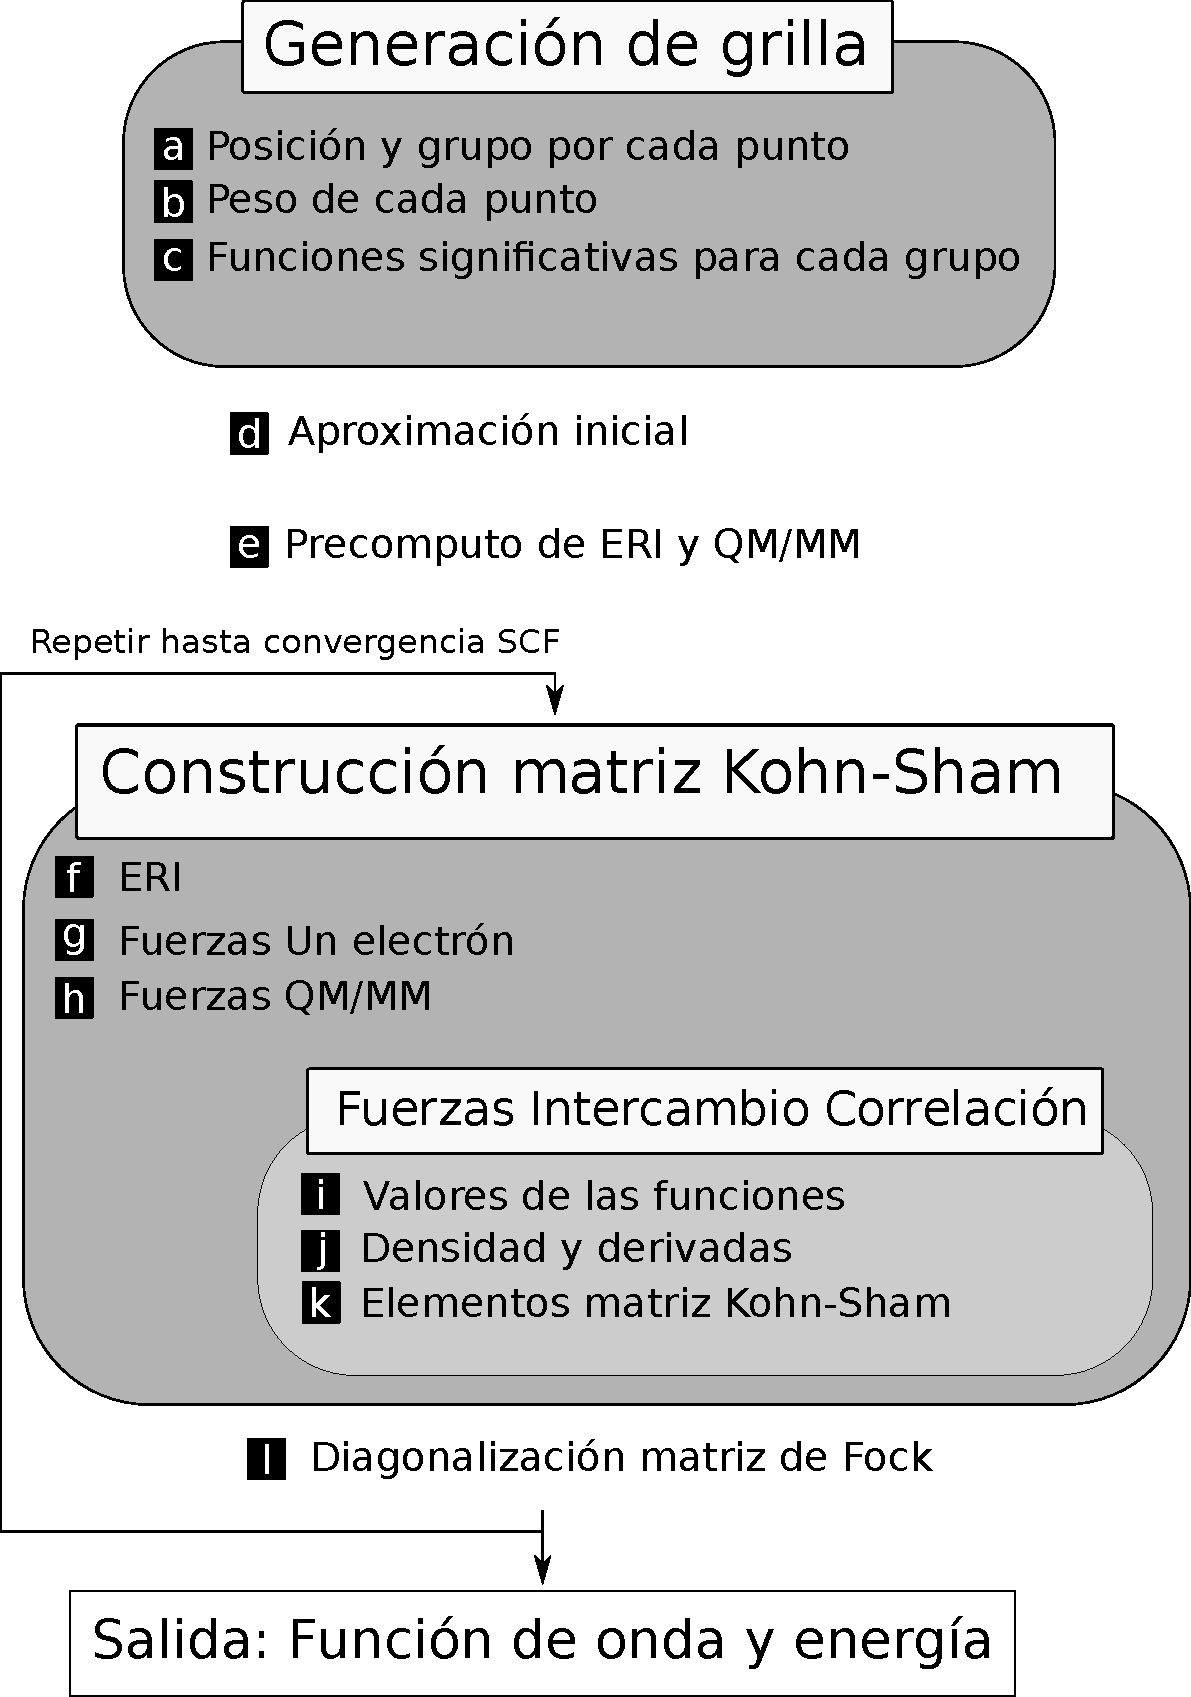
\includegraphics[width=250px]{images/g2g-steps.pdf}
   \caption{Pasos del c\'alculo de DFT realizado por LIO}
   \label{fig:lio-steps}
\end{figure}

\begin{figure}[htbp]
   \centering
   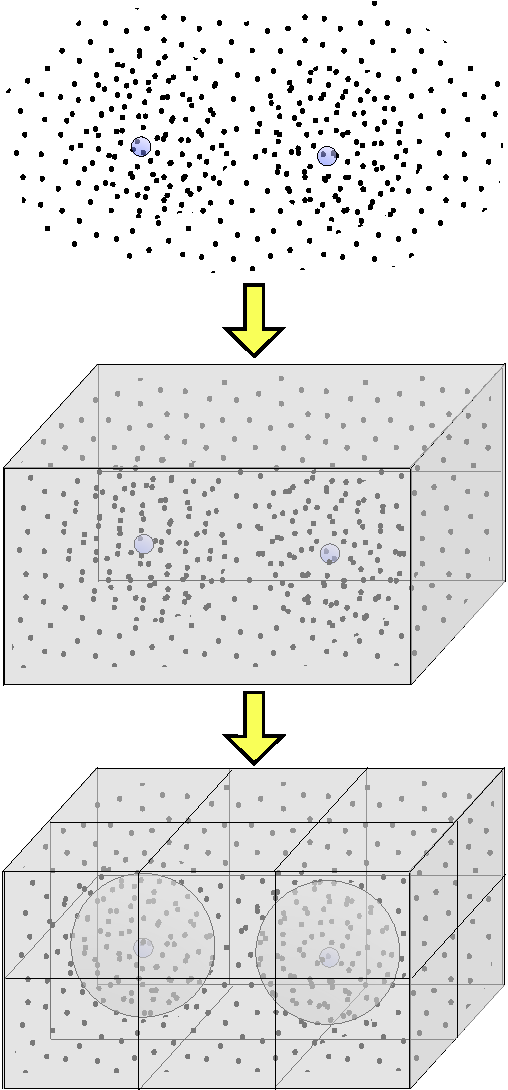
\includegraphics[width=100px]{images/grilla.pdf}
   \caption{Esquema del mallado de integracion, partido en cubos y esferas para un sistema de dos \'atomos.}
   \label{fig:grilla}
\end{figure}

Este esquema esta basado en el trabajo de Stratmann~\cite{Stratmann}, donde se propone
agrupar puntos en vez de resolver el computo uno por uno. El agrupamiento permite determinar
cuales funciones tienen una contribuci\'on significativa al computo final. Dado que las
funciones Gaussianas decaen r\'apidamente a la distancia, el tama\~no del conjunto de
funciones significativas no depende del n\'umero de \'atomos del sistema. Es decir, el tama\~no
tiene orden constante en t\'erminos de complejidad computacional. Como consecuencia, es posible
subdividir el c\'alculo de la DFT computando los grupos independientemente.

Para construir estos grupos se genera un mallado en cubos y esferas que incluya todos los puntos
de la grilla. Como los puntos no se distribuyen homogeneamente, sino que la mayor cantidad de ellos
se concentran cerca de los núcleos, si se usara una particion unicamente basada en cubos, la cantidad
de puntos contenidos en cada grupo diferiria considerablemente. El uso de grupos esféricos rodeando
los nucleos eliminan zonas de alta concentraci\'on de puntos y permite que los puntos remanentes
tengan una distribuci\'on mas homogenea. Este esquema de construcci\'on se muestra en la figura~\ref{fig:grilla}
y el detalle algoritmico de la generaci\'on se estudi\'o previamente~\cite{LIO}~\cite{TesisNitsche},
sin modificaciones para este trabajo.

Un diagrama simplificando la estructura del c\'alculo de DFT se puede ver en la figura \ref{fig:lio-steps}.
Los pasos (a) a (e) corresponden a la etapa de inicializaci\'on, y se calculan una \'unica vez
al comienzo de la simulaci\'on. La iteraci\'on de SCF (\textit{Self-Consistent Field}) se
compone de los pasos (f) a (l). Este ciclo se repite mientras la matriz densidad cambia
menos de una cierta tolerancia previamente establecida. Se agrega una condici\'on de corte ac\'a
en el n\'umero de iteraciones, para poder capturar los sistemas mal condicionados.~\cite{LIO}

Los pasos de la figura \ref{fig:lio-steps} m\'as computacionalmente costosos son (i), (j) y (k).
En la implementaci\'on original de LIO~\cite{TesisNitsche}, se muestra como estos pasos
obtienen grandes mejoras en GPU sobre su implementaci\'on de referencia en CPU. Sin embargo,
estos pasos todav\'ia insumen una gran cantidad de tiempo, incluso en las versiones aceleradas.

Estudiaremos distintos cambios hechos a las rutinas para minimizar los tiempos,
sin cambiar la estructura general del c\'alculo, ya probado en la literatura.

\section{Implementaci\'on en CUDA}

\subsection{Cuellos de botellas originales}

De las etapas descriptas en la figura \ref{fig:lio-steps}, el m\'as costoso
en la implementaci\'on existente para GPU es el paso (j). En el c\'alculo de un sistema
de tama\~no medio, este paso solo representaba el 95\% del tiempo total. Esto hacia
que esta etapa llevara tanto tiempo como todos los dem\'as c\'alculos de SCF combinados, incluso
en las GPU m\'as veloces del mercado (Tesla K40, GeForce GTX 780). Adem\'as, en Fermi
el tiempo de c\'omputo de SCF era menor que en Kepler, yendo en contra de lo que prometen
las especificaciones de estos dispositivos.

A continuaci\'on detallaremos muchos de los cambios que fueron realizados para aumentar
la performance del c\'omputo de SCF.

\subsection{Subsaturacion de los SM}
La subsaturacion de los SM se da en los casos donde haya SM que est\'en listos para correr
c\'odigo pero que no puedan hacerlo porque tienen contenci\'on en algunos de sus recursos.
La m\'etrica usada para determinar esta saturaci\'on es la ocupancia de los SP.
Esta es la proporci\'on de threads activos sobre el total de threads disponibles de un bloque.

Existen en esta arquitectura principalmente tres recursos que, en un principio, parecen
ilimitados pero en realidad son finitos y compartidos por los procesadores de la GPGPU.
Estos son:
\begin{itemize}
\item Cantidad total de threads por bloque.
\item Cantidad total de registros usados por thread.
\item Cantidad de memoria compartida por bloque.
\end{itemize}

El mecanismo de scheduling de los SM funciona asignando un bloque a cada SM, que
va a correr sin preemption hasta que terminen todos sus threads asignados. Idealmente, cada
bloque cuenta con una cantidad de threads suficiente para poder esconder la latencia
de las ejecuciones mediante un cambio de contexto. La arquitectura GPGPU esta dise\~nada
para este fin, por lo cual se cuenta con un mecanismo de cambio de contexto de costo cero~\cite{NvidiaFermi} para
poder empezar a correr los threads de un warp diferente, del mismo bloque.
Si el bloque no cuenta con suficiente cantidad de threads para poner a correr de manera
concurrente, el SM va a forzosamente esperar que finalicen las operaciones de alta latencia
de estos warps sin nada que hacer mientras tanto. Si, por el contrario, se contasen con
miles de threads por bloque, entonces es posible que las operaciones que sirvan
para sincronizar los threads de todo un bloque en un punto espec\'ifico antes de proseguir
(un barrier) sean excesivamente costosas.

La arquitectura GPGPU de \nvidia organiza los registros de todos los threads en un \'unico
register file, com\'un a todos los bloques. Como cada thread usa decenas de registros para guardar
los computos intermedios, \nvidia decidi\'o unificarlos, ya que es muy variable la cantidad que va a usar
cada kernel de ejecuci\'on. Una de las grandes diferencias entre Fermi y Kepler es la cantidad m\'axima de
registros por thread. Mientras que Fermi permit\'ia hasta 63 registros, Kepler permite hasta 255. Esto
es positivo para poder correr bloques de pocos threads pero gran cantidad de registros. Por otro lado,
aumenta la presi\'on sobre el register file. Cuando se lanzan muchos threads
que puedan estar corriendo paralelamente entre todos los SM de la GPU, es posible que se supere
la cantidad m\'axima de registros presentes en el register file. Esto fuerza a que el scheduler
no pueda poner a ejecutar m\'as bloques que los que pueda soportar este recurso, dejando SP ociosos.

Finalmente, al igual que con los registros, la memoria compartida es un recurso limitado. Como
solamente se cuenta con hasta 48KB (Fermi-Kepler) de memoria de este tipo para ser repartida entre
todos los bloques que est\'en corriendo en todos los SM, el scheduler deber\'a decidir no poner a ejecutar
m\'as bloques simult\'aneamente que los que pueda soportar la cantidad de memoria compartida.

El problema de optimizar el c\'omputo del t\'ermino de intercambio-correlaci\'on tratado  cont\'o
con todos estos limitantes. Afortunadamente,
las herramientas de profiling usadas remarcan estos limitantes, haci\'endolas
fundamentales a la hora de evaluar como proseguir en la b\'usqueda de optimizaciones de c\'odigo.

\subsection{Cambios en el threading}
%Cambiamos de blocks por puntos, a blocks por funci\'on.

De los 3 kernels que originalmente compon\'ian la iteraci\'on de SCF en GPU, el que se encargaba
del c\'alculo de la densidad electr\'onica de la contribuci\'on de la energ\'ia de intercambio correlaci\'on
insum\'ia el 94\% del tiempo total de uso de la GPU. Minimizar el tiempo de ejecuci\'on de
esta funci\'on resultaba vital para poder disminuir el tiempo de convergencia de SCF.

Este kernel computa resoluci\'on num\'erica de la integral descripta en la secci\'on introductoria.
\begin{equation}
    E_{XC} = \int \rho(r) \epsilon_{xc}\left( \rho(r) \right ) dr
\end{equation}
\begin{center}
    $\Downarrow$
\end{center}
\begin{equation}
  E_{XC} \approx \sum^{puntos}_k \rho^k \epsilon_{xc} (\rho^k,\nabla \rho^k) W_j
\end{equation}
donde
\begin{equation}
  \rho^k = \sum_{i<m} F^k_i \sum_{j<i} F^k_j C_{i,j}
\end{equation}
Esta calcula el termino de la energ\'ia de intercambio correlaci\'on, usando una grilla
de puntos con peso. Esta cuenta se realiza por cada partici\'on de los grupos en el mallado
del problema. El t\'ermino $\rho$ se obtiene de la base gaussiana usada, y $\epsilon_{xc}$
son los coeficientes variacionales. La operatoria entonces que se realiza
en el procesador es
\begin{equation}
  E_{XC} \approx \sum^{puntos} \sum_{i<m} F_i \sum_{j<i} F_j C_{i,j}
\end{equation}

Donde $F_i$, $F_j$ son los valores del mallado de las funciones de la base en un punto dado,
$m$ es la cantidad de funciones de la base y $C_{i,j}$ son los coeficientes de la matriz densidad.

El cuello de botella fundamental en la ejecuci\'on radicaba en como se distribu\'ia el trabajo de computo
entre los kernels. La estrategia de paralelizaci\'on original determinaba la partici\'on
del sistema a resolver instanciando un bloque por cada punto ({$blockId.x < m$}),
una cantidad fija de threads (usando $threadId.x < BLOCK\_SIZE$)
Los threads serv\'ian para reutilizar la memoria compartida; cada thread le\'ia un
elemento de la matriz de coeficientes ($C_{i,j})$) y luego lo compart\'ian con los
dem\'as threads.


\begin{figure}[htbp]
   \centering
   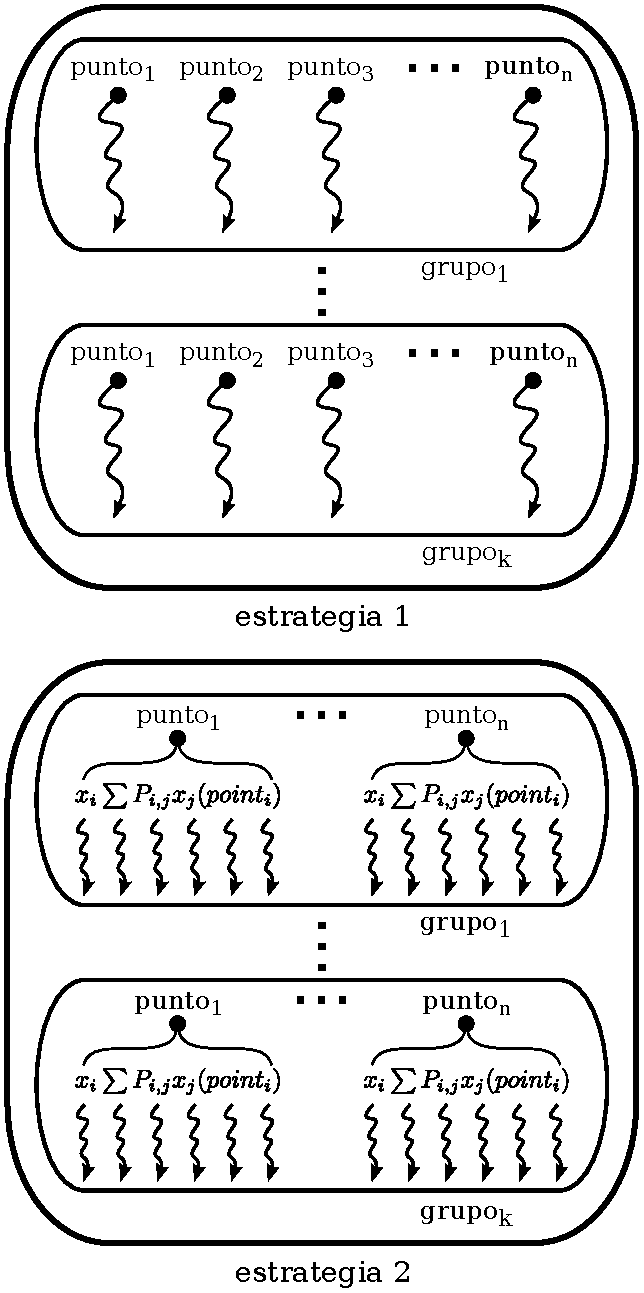
\includegraphics[width=250px]{images/cuda-parallelism.pdf}
   \caption{Estrategia original y modificada de paralelismo en el kernel de computo de la densidad
   electr\'onica computada durante $E_{XC}$.}
   \label{fig:cuda-xc-parallelism}
\end{figure}

El cambio m\'as importante para la performance provino de reconsiderar
la estrategia de partici\'on. La grilla con un bloque por punto con una cantidad
fija de threads tiene el problema de que, con bases grandes, tiene que realizar
mucho trabajo por bloque. Esto causa que los SM est\'en ocupados constantemente
por kernels de larga duraci\'on. Lo que se busca es que los  bloques realicen
menos trabajo por llamada, de modo que se puedan despachar a mas SM a medida
que estos terminen. En definitiva, lo que se busca es incrementar el throughput
de la placa. Esta estrategia se observa en la parte superior de la figura
\ref{fig:cuda-xc-parallelism}.

La nueva partici\'on que se eligi\'o dispone un bloque por funci\'on,
de modo que cada thread $i$ realice la cuenta $F_i \sum_{j}^{i} F_j C_{i,j}$
y se compartan entre threads los valores de $F_i$ le\'idos.
Esta estrategia se ve en la parte inferior de la figura \ref{fig:cuda-xc-parallelism}.

La nueva estrategia permite una mucho mayor reutilizaci\'on de las lecturas a memoria
global, uno de los grandes limitantes de esta arquitectura.
La distribuci\'on original resultaba natural al problema, pero visto en detalle, esto
implicaba una cantidad elevada de lecturas a memoria global. Como cada thread realizaba un
punto dentro de un bloque, los $F_i$ que iba a leer no se pod\'ian compartir al ser
propios de cada punto. Como la cuenta ahora se realiza parcialmente por cada thread,
cada lectura de $F_i$ se agrega a la memoria compartida. El resto de los threads no van
a leer las funciones  de memoria global, sino de la compartida que ya cargaron los dem\'as. Esto
se traduce en que se realiza una lectura global y $BLOCK\_SIZE-1$ lecturas
de memoria compartida por cada thread. Como la latencia de acceso a memoria compartida
es, al menos, diez veces mas r\'apida que la memoria global~\cite{Demystifying}, esto incurre en grandes
beneficios con respecto a la velocidad del c\'omputo.

Este cambio solo es posible gracias al crecimiento de las memorias compartidas (16KB en la generaci\'on de
dispositivos existentes en implementaci\'on original, actualmente 48KB). Finalmente
esto tambi\'en se beneficia del incremento en tanto la cantidad de SM y la de SP por
SM. Todos estos factores permitieron una gran aceleraci\'on.

El otro cambio importantes fue partir en problema en m\'as bloques para las grupos que tengan
m\'as funciones significativas. Se decidi\'o agregar otra dimensi\'on a la grilla de bloques (\texttt{blockId.y}),
para determinar cuantos grupos de threads van a hacer falta para procesar completamente
todas las funciones de ese punto. Llamamos a este par\'ametro $altura\_bloques$. Se
calcula para cada partici\'on como $altura\_bloques = {m}/{BLOCK\_SIZE}$.
Para las particiones chicas, este valor no supera a 1. En los cubos y esferas m\'as
grandes (de los sistemas probados), la altura puede ser hasta 6. Esto significa una gran
cantidad de bloques adicionales con respecto al m\'etodo anterior.

\begin{figure}[htbp]
   \centering
   \includegraphics[width=\plotwidth]{plots/cuda/threading.png}
   \caption{Aceleraci\'on en veces de correr Hemoglobina en distintas arquitecturas con el cambio de estrategia.}
   \label{plt:threading}
\end{figure}

%%
%%

Despu\'es de haber hecho el cambio de la paralelizaci\'on, estudiamos realizar
m\'as de un punto por thread. Esto sirve para aprovechar un par de lecturas que son comunes
entre dos funciones. Con este cambio, se instancian menos bloques (la mitad de la dimensi\'on $y$
definida para esto) y se pueden ocultar algunas latencias de acceso, pero
cada grupo de threads lleva m\'as tiempo y usan m\'as registros. Esta estrategia es similar
a un loop unrolling manual, aplicado a la arquitectura GPU.

Un punto de intensa discusi\'on durante estos cambios es el valor de \textit{BLOCK\_SIZE}.
Para nuestro problema, decidimos utilizar un numero de threads por bloque m\'ultiplo del
tama\~no de un warp (32 threads). Esto permite estudiar como afectan en el tiempo de
procesamiento contar con uno o m\'as warps por bloque. Una ventaja de usar bloques de
32 threads, es que el costo de la sincronizaci\'on es exactamente cero. No se precisa
sincronizar nada puesto que los threads trabajan en lock-step sincronizados por warp.
Un bloque chico ademas nos permite usar mas memoria compartida por thread, dado que hay una
cantidad fija de memoria por bloque (entre 32KB y 64KB). Cuando se cuentan con muchos m\'as
threads, se debe reducir este uso por thread de modo que todos puedan ejecutar concurrentemente.

Dicho esto, la literatura~\cite{farberCuda} sugiere siempre que sea posible
usar bloques grandes y con threads lo m\'as independientes posibles. Una gran cantidad de threads
en un bloque permite tener muchos m\'as warps para schedulear de modo de esconder las latencias de
operaciones y de a accesos globales. Sin embargo, contar con muchos threads hace que las
sincronizaciones sean mucho m\'as costosas. Ademas, como cada SM no cuenta con preemption
de bloques, contar con muchos threads por bloque hace que los recursos se mantengan
por largos periodos.

Inicialmente, este tama\~no se hab\'ia fijado en 128 threads por bloque, 4 warps. Utilizando
mas memoria compartida en el esquema de paralelizaci\'on para disminuir accesos a memoria global,
este valor resulto demasiado elevado y disminu\'ia la posibilidad de ocupar todos los SM en dispositivos
Fermi y Kepler. Con solamente 32 threads, se pod\'ia maximizar la ocupaci\'on de los SM, pero hab\'ia
muchos m\'as bloques. Finalmente, luego de disminuir un poco el uso de memoria compartida por
bloque, usando algunas ideas descriptas a continuaci\'on, pudimos fijar este valor en 64 threads
por bloque. Se muestra en la figura \ref{plt:dbs-runtime} que tener solo un warp es bueno, pero
mejor a\'un es tener dos warps corriendo simultaneamente, porque
esto permite, con costo cero, poner a correr el otro para ocultar la latencia sin agrandar
demasiado el costo de la sincronizaci\'on.

Habiendo hechas todas las dem\'as optimizaciones detalladas en las secciones siguientes, evaluamos
\'unicamente este par\'ametro. Evaluamos un bloque de 32 threads hasta 128 threads por bloque,
el m\'aximo valor posible de modo que entre nuestro uso de memoria compartida.

\begin{figure}[htbp]
   \centering
   \includegraphics[width=\plotwidth]{plots/cuda/dbs.png}
   \caption{Tiempo de ejecuci\'on del kernel density corriendo Hemoglobina variando
   la arquitectura y tama\~no de \textit{BLOCK\_SIZE}.}
   \label{plt:dbs-runtime}
\end{figure}


\subsection{Reducci\'on anterior}
%Hubo que agregar reducci\'on de suma a nivel punto porque ya no se comparten mas la info
La reorganizaci\'on de la paralelizaci\'on del kernel del c\'alculo de la densidad creo la necesidad
de varios pasos de reducci\'on que antes se hac\'ian impl\'icitamente.

El primer paso, al ya no haber un bloque por punto, habr\'a que totalizar el c\'alculo de la
suma de todos los elementos de la columna que acabamos de procesar para obtenerlo. Para reducir,
vamos a reutilizar la memoria shared que empleamos en el c\'alculo de la energ\'ia anterior. Cada
thread va a poner el valor final del computo realizado en su posici\'on correspondiente en el
la memoria compartida. Esto luego se ejecuta como una reducci\'on en \'arbol, donde cada
thread suma el valor de la posici\'on $x$ con el valor en $2*x$, si fuera este valido. Esto
luego se repite por la mitad de los threads, hasta que solo el thread 0 lo ejecuta,
generando exactamente un valor por bloque, que lo va a terminar escribiendo en la memoria
global.

Esta t\'ecnica de reducci\'on es sumamente conocida para arquitecturas distribuidas, generando
la respuesta en $O(log_2(n))$ pasos. La literatura de CUDA~\cite{cudaReductions} sugiere t\'ecnicas adicionales para
minimizar a\'un mas el tiempo empleado en esta reducci\'on, pero considerando que hay, a lo sumo
6 operaciones, no hay necesidad de mejorar esto mas.

Como va a haber $altura\_{bloque}$ cantidad de escrituras para cada punto, va a entonces
hacer falta guardar estas cuentas parciales en memoria global. Para eso definimos una matriz
por cada uno de los par\'ametros que debemos acumular, con tama\~no id\'entico a la cantidad de bloques
del kernel del computo de densidad electr\'onica, para que cada uno de estos escriba \'unicamente en una posici\'on
un\'ivocamente identificada de este. Estas matrices luego son de tama\~no $O(\#_{puntos} * altura_{bloque})$,
menos de 1MB en el caso m\'as grande.

El siguiente paso de la reducci\'on consiste en acumular los $altura\_{bloque}$ valores descriptos
reci\'en en un solo por punto. Esto implica encontrar donde est\'an en las matrices temporales las
partes de las cuentas, agregarlas y calcular el potencial correcto. Esto genera finalmente los
coeficientes para calcular la actualizaci\'on de la matriz de Kohn-Sham y los factores para el
c\'alculo de la matriz de fuerzas.

Esto se refleja en el c\'odigo como una llamada a un nuevo kernel adicional, posterior a la
cuenta de la densidad y con m\'ultiples matrices temporales adicionales. Este kernel es sumamente
eficiente porque ya todo el trabajo pesado lo hizo el anterior. Solo se tiene que realizar
a lo sumo $altura\_{bloque}$ sumas y una llamada a la funci\'on que calcula el potencial y densidad,
un kernel corto de alta intensidad aritm\'etica que realiza solamente operaciones matem\'aticas.
Finalmente, la acumulaci\'on finaliza, generando un valor por cada punto, lo mismo que se produc\'ia
anteriormente pero utilizando mucho mejor los recursos del dispositivo.


%%%%%%%%%%%%%%%

\subsection{Tama\~no de los grupos}
Un punto que afecta fuertemente el tiempo de ejecuci\'on del calculo de Intercambio Correlaci\'on
es el tama\~no de los grupos que particionan los puntos del mallado. Los grupos son generados
en base a constantes ajustables particulares a cada sistema, como se menciona en la seccion \ref{implementacion}.
Estas constantes definen el tama\~no de cada cubo y el radio de cada esfera. El impacto de
estos par\'ametros consiste en la cantidad de funciones significativas y puntos que van a ser
capturados en cada grupo. Grupos muy chicos van a contar con pocas funciones y puntos, necesitando
cientos o miles de grupos para poder representar un sistema de manera completa. Hacer grupos grandes,
en cambio, permite que tengan miles de puntos y cientos de funciones, siendo aproximadamente un orden
de magnitud m\'as grupos que en particiones chicas. Esto, sin embargo, no implica que todos
los grupos sean grandes, simplemente que los cubos y las esferas cubrir\'an espacios mayores
pero que dentro de estas puede haber pocos puntos.




\subsection{Cambios en los accesos globales}
La arquitectura de las placas de v\'ideo est\'an pensadas entorno al poder de computo.
Las decisiones tomadas por los dise\~nadores de las GPGPU se concentran alrededor
de paralelismo a lo ancho, poniendo un gran \'enfasis en la cantidad de n\'ucleos. Luego,
se dispone de menor cantidad de espacio disponible en el \textit{die} para las memorias.

Esta decisi\'on implica que la amplia mayor\'ia de la memoria de la GPGPU se encuentra
localizada externa al procesador.  No solo esta f\'isicamente mas lejos, sino que
adem\'as la latencia para accederla es muy elevada. Es decir, el paradigma de
programaci\'on de las GPGPU gira entorno a esconder la gran latencia de los accesos
a las memorias globales.

As\'i como en CPU es importante realizar accesos alineados a memoria, en GPU es aun m\'as cr\'itico.
El termino coalescencia de memoria se define en GPU como la organizaci\'on de los accesos a memoria de secuencial, ordenada y predecible.
La l\'ogica detr\'as de esto es que cuando el GPU accede a memoria de manera alineada, puede traer 16, 32 o 64 elementos de 32 bits en una sola lectura, suficiente para
cada uno de los threads del warp. Si, en cambio, debe acceder de manera no
alineada a memoria o con threads que no acceden de manera predecible, entonces
se deber\'an serializar los accesos y separar en m\'ultiples transacciones a memoria global para satisfacer
el pedido. Este problema se agrava si se debe hacer accesos frecuentes
por cientos de threads, como es el caso de los bloques con gran nivel de paralelismo explicito.

En el paso del c\'alculo de la densidades el acceso a las funciones calculadas
se realizaba por columnas en vez de por filas. Esto ocasionaba que por cada acceso,
un warp tuviera que realizar 32 accesos secuenciales a memoria, ya que no se pod\'ian alinear
en una transacci\'on. Esto, ademas, se realizaba para las funciones, las derivadas y los
hessianos, por lo cual los accesos eran sumamente costosos. En el kernel original este comportamiento
no suced\'ia, ya que todos los threads realizaban cuentas para puntos independientes y no se compartian las
lecturas de las matrices. Esto aprovechaba las dimensiones originales de las matrices y hacian que las lecturas de
funciones fueran menos costosas, ya que se las usaba en el sentido correcto de la memoria (por filas).
Al haber cambiado la cuenta realizada para aprovechar mejor el threading (descripto en las secciones anteriores),
los accesos pasaron a ser por columnas y no por filas, rompiendo la coalescencia de las matrices. El
problema de los accesos se suele mitigar en CPU con el uso de las cach\'e, pero como las GPU cuentan
con L1 y L2 muy peque\~nas, el costo de acceder desalineado sigue siendo elevado.

Esto se soluciona transponiendo las matrices de valores de funciones, gradientes y hessianos.
La transposici\'on de matrices es un ejemplo sumamente estudiado por la literatura de CUDA
ya que ataca un punto d\'ebil de la arquitectura, el ancho de banda de transferencia. En la figura
\ref{plt:transpose} podemos ver que tanto en Fermi como en Kepler es muy notoria la diferencia
de performance, simplemente repensando los accesos a memoria. Kepler, al contar con una cach\'e L2
del doble de tama\~no que Fermi, lo mitiga un poco mas los accesos desalineados, pero todav\'ia recibe
grandes mejoras.

%Una cosa a tener en cuenta, pensando con respecto a la secci\'on anterior donde discutimos
%el cambio del threading, es que adem\'as se disminuyeron los accesos de lectura a las matrices de funcion.
%Al compartirlas entre threads usando las memorias shared, ahora se realizan muchos menos accesos a memoria global,
%ya que cada thread BLOCK\_SIZe elementos de cada matriz de funciones, pero todos salvo uno los leen de
%memoria compartida, ordenes de magnitud mas r\'apida que la global. Es decir, el impacto de este cambio
%es tan o m\'as importante a\'un que la coalescencia

\begin{figure}[htbp]
   \centering
   \includegraphics[width=\plotwidth]{plots/cuda/transpose.png}
   \caption{Aceleraci\'on en veces del kernel density de correr Hemoglobina en distintas arquitecturas habiendo transpuesto las matrices
   de funci\'on (incluyendo el costo de transponerlas).}
   \label{plt:transpose}
\end{figure}

Otra de las t\'ecnicas con la que cuenta CUDA para mitigar la latencia de acceso a memoria
es mediante el uso de memorias intermedias entre el procesador y la memoria global. Una de ellas es
la cach\'e de textura (siendo la otra la memoria constante). Esta es una cach\'e que
esta focalizada alrededor de los accesos a memoria de varias dimensiones.
Estas memorias reciben su nombre de su funci\'on principal, que es en el \'area de las
aplicaci\'ones de render de video. Los mapas de textura suelen ser grandes matrices que definen
tanto los colores sobre las superficies de los pol\'igonos como los relieves.
El detalle crucial de estas memorias es que un miss en estas cach\'e, provoca
que se traigan datos no solo contiguos en memoria, como pasa en las caches de
CPU normalmente, sino que ademas se traigan los datos en posiciones l\'ogicas contiguas,
es decir, variando las distintas dimensiones de la matriz subyacente.

Las memorias de textura se ajustan bien a los problemas de GPGPU, porque se relacionan
\'intimamente con los los mecanismos de paralelismo de CUDA. Como los problemas se pueden
dividir en bloques con threads en $x$, $y$, $z$, entonces tiene mucho sentido pensar
que las estructuras de datos subyacentes se van a acceder usando indices multidimensionales.

En nuestro problema, la memoria de textura se presenta como una soluci\'on para
los accesos bidimensionales de la matriz densidad para el grupo de puntos.
Como esta matriz debe ser multiplicada por todos los valores de las funciones,
derivadas primeras y segundas, se va a acceder a toda la matriz de coeficientes mas de
una vez por cada thread. Adem\'as, como se va a usar toda la matriz, y esta suele
tener un tama\~no intermedio (es muy grande para memoria constante), el problema
suele entrar casi completamente en la memoria de textura.
La lectura bidimensional en este caso, se ajusta muy bien a los accesos por filas
y por columnas a la matriz.

\begin{figure}[htbp]
   \centering
   \includegraphics[width=\plotwidth]{plots/cuda/texture.png}
   \caption{Aceleracion del c\'alculo de densidad corriendo Hemoglobina en Fermi y Kepler
   usando memoria de textura para leer la matriz densidad.}
   \label{plt:texture}
\end{figure}

Como podemos ver en la figura~\ref{plt:texture}, esta optimizaci\'on aprovecha este
recurso \'unico de GPU. Sin embargo, esto agrega un factor mas que tenemos que tener en
cuenta a la hora de profilear el c\'odigo. Para administrar los accesos a
la memoria de textura, cada multiprocesador tiene m\'ultiples unidades de textura.
Cuando dependemos de sobremanera de la memoria de textura para esconder la latencia,
se presentan contenciones sobre el acceso a estas unidades. Esta cach\'e hay que usarla
solamente en los accesos mas costosos \'unicamente, ya que si intentamos pasar todos
los accesos a trav\'es de este, no solo no se ver\'ian mejoras, sino que seria un retroceso
completo de performance, como sucedi\'o cuando se intent\'o agregar adem\'as las matrices
de funciones a este m\'etodo.

%http://www.realworldtech.com/gt200/10/   << detalles sobre texture cache invalidation

%\subsection{Cambios en los pasajes de informaci\'on intrawarp}
%%Los shuffles que no anduvieron salvo en function
%La arquitectura SM35, junto con CUDA5, trajeron aparejadas una herramienta interesante
%para el manejo interno de los pasajes de informaci\'on intra-warp durante la ejecuci\'on.
%Las instrucciones de shuffle, como asi las denomina \nvidia, son instrucciones que facilitan
%el pasaje directo de un registro de un thread en un warp, a otro, en un solo ciclo de ejecuci\'on.
%Estas instrucciones existen en diversas maneras, con distintos propositos. Principalmente se
%utilizan para pasar de un thread al siguiente (modulo el warp size) un registro para poder seguir
%operando. Otro uso que puede tener mucho interes proximamente son las instrucciones de votaci\'on,
%donde se evalua un predicado para todos los threads, y se setea o limpia un bit en el resultado
%de respuesta si se cumplio el predicado para ese thread. Con esta herramienta, no es necesario
%acceder a memoria compartida para poder pasar minima informaci\'on dentro de cada warp.
%
%Nuestro uso de las funci\'ones de shuffle consistio en intentar eliminar lo m\'as que podiamos
%los accesos a la memoria compartida, una fuente de bloqueos porque, a pesar de que ya corre
%todos los bloques concurrentemente, leer elementos de ahi toman 4 ciclos en vez de uno solo
%como en las funci\'ones de shuffle.
%
%Probamos pasar de a un elemento y de a uno o dos vectores de 3 elementos, para comparar
%cuan notable era el impacto del acceso mas veloz.
%
%Finalmente concluimos que era una opcion valida para el pasaje de los valores de la funci\'on,
%pero que el overhead de uso para cosas como los hessianos de la funci\'on no justifica el uso.
%Adem\'as, como estas funci\'ones de shuffle solo estan presentes en las ultimas placas Kepler,
%consideramos que el aprovechamiento marginal de los recursos no era lo suficientemente meritorio
%de romper compatibilidad con las placas de la generacion Fermi anterior.


\subsection{Cambios en el almacenamiento de matrices temporales}
Una de las principales limitaciones de las GPGPU es la cantidad fija de memoria. Esta no se puede
expandir dado que esta soldada a la placa. Esto era aun m\'as notorio cuando las placas
contaban con menos de 1GB de memoria (A\~nos 2007-2008).
Para problemas de c\'alculo num\'erico, esto era un limitante muy serio; los problemas que
normalmente entraban en la memoria principal de un CPU, no entraban completos en las GPU.
La decisi\'on tomada por muchas aplicaciones de entonces es compensar esto calculando
datos intermedios y tir\'andolos al final; teniendo que ser recalculados en las pr\'oximas iteraciones.

Esta estrategia es claramente impr\'actica en CPU, puesto que se cuenta con mucha m\'as memoria
de uso general. En GPU era necesario por el faltante de memoria, pero puesto que estas cuentas se pueden
hacer m\'as r\'apido que en CPU, convirti\'endose entonces en una estrategia valida.

Cuando la aplicaci\'on original se concibi\'o, no hab\'ia siquiera placas GPGPU apuntadas a HPC, con
m\'as memoria disponible que los modelos de consumidores. Aprovechando estos recursos actuales,
desarrollamos un m\'etodos para poder almacenar las matrices de los valores de funciones y sus derivadas
en cada punto para cada grupo durante la ejecuci\'on de la aplicaci\'on, de modo de poder aprovechar
este recurso que originalmente era limitante pero ya no. Estas incluyen la matriz de funciones,
con una cantidad de elementos $O(puntos \times funciones)$, y si se usa el m\'etodo GGA
(\textit{Generalized Gradient Approximation}) para realizar los c\'alculos de DFT, tambi\'en se requieren
las matrices de gradientes y hessianos de las funciones ($O(3 \times puntos \times funciones)$ y
$O(6 \times puntos \times funciones)$ respectivamente).

Para poder determinar que cosas van a ser guardadas en memoria y que no, se determin\'o una heur\'istica
que define el orden de las particiones a solucionar. Esta heur\'istica estima que tama\~no van a
tener las matrices temporales a almacenar y ordena las particiones de menor a mayor. Esto
esta basado en el criterio de que, si bien es proporcional el tiempo de computo de estas matrices
temporales a la cantidad de funciones por grupo y cantidad de puntos (lo que determina el tama\~no
de la partici\'on), la constante es elevada. Determinamos entonces que es m\'as conveniente
aprovechar la memoria de la placa que almacena muchas matrices temporales de particiones chicas
a que almacene solamente un par de las grandes.

Para controlar la administraci\'on de memoria, se calcula si la placa dispone
con la suficiente memoria libre para guardar las matrices de funciones, y si puede, se almacenan de manera
permanente (hasta que la partici\'on se mueva a otro dispositivo o la liberaci\'on de recursos al
finalizar las iteraciones de SCF). Este mecanismo adem\'as es configurable de modo que una ejecuci\'on
pueda usar un porcentaje de la memoria con la que cuenta la placa, para poder correr m\'ultiples procesos de
simulaci\'on concurrentemente.

Un detalle a tener en cuenta es que, incluso si se maximiza el porcentaje de memoria usado para
cachear estas matrices, tal vez no alcanza para que quepa todo el sistema evaluado en memoria. Esto
se nota principalmente en la linea GeForce, que cuentan con aproximadamente entre un cuarto y la mitad
de la memoria global que tienen su equivalente en la linea Tesla. Esto es mitigado cuando se computa
m\'ultiples placas, que tambi\'en distribuyen el almacenamiento ademas del computo.

Evaluamos el tiempo de ejecuci\'on de un sistema modelando un fullereno $C_{60}$, variando la
cantidad de memoria disponible para el cacheo.

\begin{figure}[htbp]
   \centering
   \begin{subfigure}[b]{\plotwidthtres}
     \includegraphics[width=\plotwidthtres]{plots/cuda/global-detailed-fullereno.png}
     \caption{Entre 0 y 530 MB.}
   \end{subfigure}
   \begin{subfigure}[b]{\plotwidthtres}
     \includegraphics[width=\plotwidthtres]{plots/cuda/global-fullereno.png}
     \caption{Entre 0 y 4240 MB.}
   \end{subfigure}
   \caption{Aceleraci\'on del c\'alculo de una iteraci\'on de SCF en funci\'on de la memoria libre de
   la placa usada para almacenar las funciones.}
   \label{plt:global-fullereno}
\end{figure}

Como se puede ver en la figura \ref{plt:global-fullereno}, el
almacenamiento de las matrices de funciones produce una mejora de casi el 25\% en el tiempo de ejecuci\'on
de toda una iteraci\'on de SCF. Es interesante notar que son los primeros grupos los que causan mayor
diferencia en los tiempos de ejecuci\'on. Con 5.3 MB, se pueden guardar los 23 grupos mas peque\~nos del
fullereno $C_{60}$; de ah\'i en m\'as, el impacto de la mejora decae. Esto sucede porque en grupos
chicos el overhead del c\'alculo usando kernel de funciones es muy elevado en comparaci\'on a las
cuentas (se desperdician muchos threads). Este comportamiento se puede ver
bien en en la figura~\ref{plt:runtime-functions-fullereno}, donde se puede apreciar el importante
peso de los grupos chicos en el tiempo total del c\'alculo de las funciones. Decidimos no intentar
optimizar el c\'alculo ya que al almacenar las matrices este costo directamente se hace cero para
casi todos los grupos (dependiendo si el sistema entra entero o no en memoria).

\begin{figure}[htbp]
   \centering
   \includegraphics[width=\plotwidth]{plots/cuda/global-functions-acc.png}
   \caption{Fracci\'on del total del tiempo de c\'alculo de las matrices de funciones en una iteraci\'on en funci\'on
   del ordenada por el tama\~no acumulado de estas en un fullereno $C_{60}$.}
   \label{plt:runtime-functions-fullereno}
\end{figure}

Esta simple mejora permite explotar el hecho de que las placas hayan aumentado dram\'aticamente su
capacidad de almacenamiento, un recurso que hasta recientemente venia siendo un limitante podemos
convertirlo en una aceleraci\'on notoria.

\subsection{Cambios en las memorias compartidas}
%Cambiar los vec\_type4 por 3 en los accesos a la shared es mucho mejor, no hace falta alinear ahi
Otro de los problemas existentes del c\'odigo que quisimos atacar fue el mejor empleo de las
memorias shared. Estas son un recurso finito y muy importante, ya que son un limitante de
la ocupancia de los multiprocesadores. Como pueden correr una cantidad de bloques que, a lo sumo,
no superen los 48KB de memoria shared simult\'aneamente entre todos, es imprescindible minimizar
el uso de la memoria shared de modo que no estemos subutilizando los SM.

Una cosa que probamos, con un grado de \'exito variable, fue disminuir el tama\~no de los vectores
donde almacenamos las derivadas direccionales. Como nuestro problema es en tres dimensiones,
y los vectores estaban configurados para tener 4 valores por cada derivada, probamos llevarlos a
3, para que se ajusten a su consumo real de memoria. Este acercamiento no consider\'o el porque
se hizo as\'i de esta manera originalmente. Tener 4 valores consecutivos en memoria fuerza
al compilador a alinearlos a 16/32 bytes (simple y doble precisi\'on).
Esto presenta grandes ventajas a la hora de hacer transferencias de memoria global en los accesos,
por lo cual decidimos dejarlo como estaban.

Sin embargo, este mismo criterio no aplica a las memorias shared de la GPGPU. Como los accesos
a estas memorias se realizan de a 4 bytes y no de a 16/32, entonces no tiene ninguna ventaja
en particular realizar el alineamiento; ya est\'an alineadas porque los elementos de cada punto
son flotantes de precisi\'on simple o doble (4 y 8 bytes respectivamente). Adicionalmente, como el
cuarto valor no tiene forma de marcarse como algo que no sea padding de alineaci\'on, todav\'ia se
opera normalmente con el, por lo que eliminarlo ahorra una operaci\'on de c\'alculo. Mas a\'un,
se presentan una disminuci\'on del 25\% de los recursos de la memoria compartida por thread,
sin ninguna desventaja a la hora de acceder a estos. Principalmente esta mejora, en teor\'ia, permite
aumentar la cantidad de bloques corriendo concurrentemente en los SM, para poder eliminar
la limitaci\'on presente debido al uso simultaneo de memoria compartidas.

\begin{figure}[htbp]
   \centering
   \includegraphics[width=\plotwidth]{plots/cuda/shared-4vs3.png}
   \caption{Aceleraci\'on obtenida en Fermi y Kepler al reducir a 3 componentes los
   elementos en la memoria compartida.}
   \label{plt:shared4vs3}
\end{figure}

Como se puede observar en la figura~\ref{plt:shared4vs3}, se obtienen muy pocas ganancias al usar elementos
de 3 componentes con respecto a usar elementos de 4. Esto muestra que el limitante de concurrencia
de este kernel no pasa por falta de memoria compartida. Adem\'as, esto permite apreciar que los
tiempos de acceso a los datos en las memorias shared son realmente muy bajos, pudi\'endose ver
como con incluso un 25\% mas de operaciones de lecto-escritura, el tiempo de ejecuci\'on casi no varia.


%\subsection{Cambios en los condicionales}
%La arquitectura CUDA representa un modelo de computo pensado en el procesamiento secuencial masivo
%de datos de punto flotante. Esto es herencia de su legado de placa gr\'aficas, que era un stream
%constante de datos. Al generalizar la arquitectura para que sea de prop\'osito general, entonces
%surge el problema de ejecuci\'on condicional. Como el resultado de la evaluaci\'on puede ser distinto
%para cada thread, entonces surge el problema de como ejecutar un warp en lockstep cuando algunos threads
%correr\'an la rama \texttt{true} y otros la rama \texttt{false}. La soluci\'on que adopta CUDA es la
%serializaci\'on impl\'icita. Los threads que no ejecutan el \texttt{true} correr\'an \texttt{NOP}
%y lo mismo se har\'a en el caso del \texttt{false}, al rev\'es.
%
%Esto trae aparejado una penalidad importante. Si esa bifurcaci\'on contiene mucho c\'odigo no trivial,
%entonces es evidente que se subutilizan importantemente los recursos disponibles.
%
%Habiendo varios de estos casos en los kernels presentes, decidimos utilizar una t\'ecnica sugerida
%por \nvidia. Esta consiste en hacer las operaciones normalmente, como si todos los threads cumplieran
%las condiciones del condicional y multiplicar por 1 o por 0 al resultado antes de acumular.
%Esto hace que las cuentas que no se ejecutaban antes ahora lo hagan pero que simplemente no aporten
%a la reducci\'on. Esta t\'ecnica elimina la existencia de la rama falsa de los condicionales, pero
%trae aparejada dos problemas no triviales.
%
%Uno de ellos es como solucionar el problema de los indices en los accesos a memoria.
%Un uso usual delas guardas condicionales es para evitar que el programa, si cumple ciertas condiciones,
%no acceda a memoria que esta mas all\'a de los limites definidos.
%Por ejemplo, si \texttt{threadId > arraySize}, entonces claramente
%no deber\'ia acceder a ninguna posici\'on mas all\'a de \texttt{array[threadId]},
%puesto que seria memoria invalida. Si eliminamos la guarda
%entonces los accesos a memoria pueden no quedar igual. Una soluci\'on consiste en multiplicar tambi\'en
%por 1 o por 0 la direcci\'on a la cual se va a acceder. Como CUDA maneja los arreglos de memoria
%como C (es decir, basados en 0 como primer direcci\'on), esta t\'ecnica es v\'alida para hacer
%siempre accesos correcto a memoria. El problema luego es en la coalescencia; como ahora algunos
%threads de un warp van a acceder a una posici\'on de memoria muy distinta a otros, entonces el procesado
%va a partir esos accesos en m\'ultiples transacciones. Esto puede hacer que la cuenta no solo no mejore
%la performance, sino que puede que la empeore sustancialmente. Se debe hacer un profiling caso
%por caso para poder estudiar el impacto en el kernel.
%
%El otro problema es en cuentas que pueden dar NaN (como el t\'ipico caso de divisi\'on por cero).
%Como, por est\'andar IEEE 754, los NaN hacen que todas las operaciones con ellos den NaN,
%entonces pueden propagarse por la cuenta, incluso en con multiplicaci\'on con cero del resultado.
%La soluci\'on m\'as evidente seria comprobar si son NaN antes de reducirlas, y si lo fueran, reemplazarlos
%por cero. Esto puede llegar a ser inevitable en muchos casos; en el nuestro, con replantear las cuentas,
%podemos evitarlos.

\subsection{Escalando m\'as all\'a de un GPU}
Una vez que fueron solucionados muchos limitantes de performance en los kernels del computo
de la densidad electr\'onica y del c\'alculo de la matriz de Kohn-Sham, nos encontramos en un punto donde
no fue posible determinar mejoras significativas en el c\'alculo para reducir tiempos.
Decidimos subir un nivel m\'as el paralelismo, de modo de poder solucionar m\'ultiples particiones
simult\'aneamente. Dado que es independiente el computo de cada partici\'on (salvo la acumulaci\'on
en la matriz de Kohn-Sham de salida y en la matriz de fuerzas interat\'omicas), nos pareci\'o que seria
interesante ver como escala distribuir el computo a lo largo de m\'ultiples GPU.

Para dividir el problema entre varios dispositivos usamos, al igual que en CPU, OpenMP. Definimos
una secci\'on paralela dentro del loop principal donde se soluciona cada grupo de modo que se
ejecutaran tantos threads como placas haya en la maquina. Cada
uno de los threads en el host se configurar\'a para una placa solamente. Esto se realiza con
una instrucci\'on del driver de CUDA (CudaSetDevice) que permite que durante toda la vida del
thread, todas las llamadas a kernels se realicen autom\'aticamente al mismo dispositivo.

CUDA permite que trabajar con m\'ultiples placas de esta manera sea bastante sencillo. Las variables
definidas como \texttt{\_\_device\_\_}, que residen plenamente en la GPU, son autom\'aticamente instanciadas
por cada dispositivo presente. De esta manera, es impl\'icito cual variable usa cada kernel; la que
esta definida para su dispositivo actual. Esto puede ser un problema si queremos lograr comunicaciones entre placas,
pero si las cuentas son independientes, es paralelismo gratuito de costo cero.

El principal problema que surge de uso de m\'ultiples dispositivos radica, al igual que en
CPU, en como distribuir la carga de los threads de modo tal que haya una cantidad de trabajo
similar, para minimizar los tiempos de idle. Este problema no es tan grave siempre y cuando
se utilicen placas id\'enticas dentro de la configuraci\'on del sistema ya que seria
el mismo tiempo si se corre en una o en otra. Un trabajo adicional de inter\'es ac\'a
radicar\'ia en el uso de t\'ecnicas de estimaci\'on de poder de computo para poder
distribuir el trabajo de manera equitativa entre modelos de placas heterog\'eneas, con distintas
configuraciones de memoria, cantidad de SM y anchos de banda.

Para distribuir las tareas utilizamos dos t\'ecnicas combinadas, una para distribuir las
tareas est\'aticamente y otra para redistribuirlas din\'amicamente de acuerdo al runtime de
cada tarea.


\subsubsection{Estimaci\'on de cargas est\'aticas}
Para la distribuci\'on est\'atica, usamos como estimador del runtime el tama\~no
de las matrices de funciones de un grupo. Esta heur\'istica resulta un acertado predictor
del tiempo de computo de todos los
kernels de un grupo confirmando que el problema actualmente es memory-bound. Esto se ve en la figura
\ref{plt:runtime-predictor}, como el tiempo de resoluci\'on de un kernel escala linealmente con
la cantidad de memoria necesaria para operar. Comparamos tambien contra el predictor usado
para estimar tiempo en CPU que se detallar\'a m\'as adelante en la secci\'on \ref{PredictorCPU}.

\begin{figure}[htbp]
   \centering
   \begin{subfigure}[b]{\plotwidthtres}
    \includegraphics[width=\textwidth]{plots/cuda/sizeingpu-predictor-hemo.png}
     \caption{Predictor de tiempo usando \textit{size\_in\_gpu}.}
   \end{subfigure}
   \begin{subfigure}[b]{\plotwidthtres}
    \includegraphics[width=\textwidth]{plots/cuda/cost-predictor-hemo.png}
     \caption{Predictor de tiempo usando funci\'on de costo.}
   \end{subfigure}
   \caption{Tiempos de ejecuci\'on de hemoglobina en Tesla K40 de acuerdo al costo del mismo seg\'un predictor.}
   \label{plt:runtime-predictor}
\end{figure}

Como podemos apreciar, esta directamente relacionado el tiempo de resoluci\'on con el tama\~no
de los elementos con los que trabaja. Esto da una pauta de la complejidad computacional del problema
que estamos resolviendo. Como al menos se necesita cada uno de los elementos de cada matriz de funciones
para resolver un punto de cada grupo. Al menos se deben hacer una lectura de cada matriz. Estas lecturas
son tan costosas que, incluso solo sabiendo el tama\~no de las matrices, podemos predecir aproximadamente
el tiempo de ejecuci\'on que va a tener un grupo.

El predictor usando el tama\~no, si bien es posible observar que tiene una buena correlaci\'on con el tiempo de ejecuci\'on,
no tiene la precisi\'on que tiene el predictor basado en la funci\'on de costo en CPU, visto en la figura~\ref{fig:comp-size-cost}.
No se pudo encontrar par\'ametros que permitan ajustarlo para que funcione en GPU. Como \nvidia no publica toda la informaci\'on
interna de los procesadores GPU y dada la cantidad de lugares adicionales donde se puede incurrir en latencias
imprevistas, al funcionar as\'incronos al CPU, no es posible predecir runtime con excesiva confianza dado \'unicamente
las cuentas a realizar. Al tener ambos predictores performance similares, se decidi\'o usar el m\'as sencillo, el
tama\~no de la matriz, como punto de partida para realizar una partici\'on del sistema en m\'ultiples GPU.

\subsubsection{Balance de cargas}
El balanceo de cargas \'optimo consiste en repartir $P$, el conjunto de problemas en
$n$ conjuntos disjuntos $P_i$, tal que $\bigcup_{i<n} P_i = P$. Este problema, conocido como PARTITION,
es NP-Hard en su versi\'on exacta, aunque son conocidos algoritmos pseudo-polinomiales para resolverlo.
La complejidad de ese algoritmo que usa programaci\'on din\'amica es $O(Nn)$, con $N$ el valor
de la suma de $P$ y $n$ la cantidad de elementos de $P$. Como nuestra m\'etrica de comparaci\'on para las
particiones es el runtime de estas expresados con precisi\'on de microsegundo, el costo computacional
de este algoritmo puede ser elevado en sistemas con cientos de particiones de miles de puntos.
La principal desventaja de usar \'unicamente este algoritmo es que no contempla, o no al menos
en sus versiones m\'as directas, el uso de recursos asim\'etricos. Es decir, resolver la partici\'on
optima del problema de particiones cuando se sabe que el costo de resolver $P_i$ en el dispositivo
$A$ es distinto a resolverlo en el dispositivo $B$. Por este motivo, no podemos particionarlo completamente
de manera est\'aticamente
usando este algoritmo y decidimos agregar usar una soluci\'on h\'ibrida est\'atica y din\'amica, reutilizando
la informaci\'on de runtime para decidir como rebalancear las particiones entre iteraciones de SCF, luego
de haber hecho una aproximaci\'on inicial usando el predictor est\'atico antes mencionado.

Inicialmente definimos un orden para realizar toda la resoluci\'on del sistema y
se las distribuye de manera \textit{round-robin} entre todos los dispositivos, para generar la
partici\'on inicial y cargando a cada placa con una cantidad similar de tareas. Esto no significa
que todas tarden lo mismo, y es posible notarlo en las mediciones. Luego, utilizando el tama\~no
de los dispositivos como proxy del tiempo de ejecuci\'on, aplicamos una ronda del algoritmo de balanceo din\'amico
para terminar de balancear est\'aticamente. Esto lo podemos hacer ya que, como mostramos en la figura~\ref{plt:global-fullereno},
existe una fuerte correlaci\'on entre el tama\~no de las matrices de funci\'on y el tiempo de ejecuci\'on, la m\'etrica que realmente
nos interesa. El paso de balanceo din\'amico es necesario para solventar el problema de la distribuci\'on
round-robin con grupos grandes, donde el thread que tenga que resolver el grupo con mas puntos va a tardar
desproporcionadamente mas que los dem\'as. Un caso emblem\'atico es el cubo que contiene al \'atomo de hierro en la hemoglobina,
con mas de diez mil puntos y cientos de funciones de la base, con un tiempo de ejecuci\'on de al menos
dos ordenes de magnitud mas que el mas chico.

Para hacer el balanceo din\'amico, debemos determinar de ante mano la performance de cada
dispositivo con el que contemos. Para esto, se usa la tradicional t\'ecnica de definir un
caso de prueba representativo del problema, ejecutarlo en cada uno de los dispositivos y anotar
cuanto tarda en cada uno de ellos. Una gran ventaja de esto es que permite balancear f\'acilmente las
cargas cuando se realizan operaciones de doble precisi\'on en conjuntos de dispositivos que incluyan
placas Tesla y placas GeForce. En simple precisi\'on, los topes de linea de cada una pueden tener
performance similares (por ejemplo, GTX 580 y M2090, GTX 780 y K20), pero en doble precisi\'on
usualmente las Tesla suelen ser entre 2 y 6 veces mas veloces. Como las cuentas se realizan
o todas en precisi\'on simple, o todas en precisi\'on doble, es sumamente importante particionar el
sistema tomando todo esto en cuenta.

El problema ejemplar elegido en este caso es realizar $10$ iteraciones del kernel de c\'omputo de la matriz de Kohn-Sham.
Consideramos que realizar este c\'omputo nos da una evaluaci\'on
emp\'irica de los recursos necesarios para resolver este problema. Este kernel utiliza muchos
de los recursos del dispositivo: realiza gran cantidad de accesos a memoria a trav\'es
de la unidad de textura, usa principalmente instrucciones FMA, tiene una m\'axima ocupaci\'on de los SM
y tiene un uso total de la memoria shared. No contabilizamos las copias de memoria desde y hacia la
placa de los par\'ametros puesto que, al igual que en el c\'odigo de la simulaci\'on, casi la totalidad
de los datos se construyen directamente en la placa y se recuperan las matrices reducidas solamente al final
de la operaci\'on.

Teniendo las mediciones de tiempo para los $d$ dispositivos disponibles, se construye la matriz de
correcci\'on de tiempos de ejecuci\'on con los $d^2$ los coeficientes de correcci\'on para poder estimar el tiempo de
ejecuci\'on en el nuevo dispositivo. Si los dispositivos presentes son id\'enticos, como suele ser el caso
en clusters de computo cient\'ifico, entonces
la matriz va a tener solamente valores muy cercanos a 1, l\'ogicamente.

El pseudo c\'odigo del algoritmo de balanceo se detalla a continuaci\'on.
\begin{algorithm}
  \caption{Balanceo de duraci\'on de threads}
  \label{ThreadBalancing}
\begin{algorithmic}
  \State $tiempo_{\min} \gets duracion[T_{\min}]$
  \State $tiempo_{\max} \gets duracion[T_{\max}]$

  \While {$tiempo_{\max} < tiempo_{\min} * k$}
    \State $\Delta T \gets (tiempo_{\max} - tiempo_{\min}) /2$
    \ForAll{$G_i \in Trabajos[T_{\max}]$}
    \If{$duracion[G_i] * correccion[T_{\max}][T_{\min}] * penalidad\_migracion - \Delta T < duracion[{G_{mejor\_candidato}}]$}
        \State $G_{mejor\_candidato} \gets G_i$
      \EndIf
    \EndFor
   \State Liberar la memoria de las marices cacheadas de $G_{mejor\_candidato}$
   \State Mover $G_{mejor\_candidato}$ de $T_{\max}$ a $T_{\min}$
   \State Actualizar la duraci\'on total de $T_{\max}$ a $T_{\min}$, aplicando la correcci\'on de tiempos
  \EndWhile
\end{algorithmic}
\end{algorithm}

En el algoritmo \ref{ThreadBalancing} se definen dos constantes adicionales, $k$ y $penalidad\_migracion$.
$k$ representa el coeficiente de m\'axima diferencia de tiempo entre el thread de mas larga duraci\'on y el de menor
duraci\'on. Para nuestros usos, un valor de $k \approx 2\%$ es aceptable.
$penalidad\_migracion$ es un coeficiente que agrega un costo al migrar el grupo a otra placa, ya que va
a tener que recalcular las matrices que ya se guardaba en memoria. Cuando cambie de placa, va a tener
que desalojarlas ya que, si bien es posible que entre las placas se accedan mutuamente a memoria global (utilizando
el direccionamiento unificado introducido en CUDA 5)
no conviene dada toda la latencia introducida, que se adicionar\'a a lo largo de todas las iteraciones de la resoluci\'on.
Este coeficiente es equivalente a definir una penalidad por romper la \textit{afinidad} de las caches en CPU.

%Adicionalmente, el algoritmo \ref{ThreadBalancing} agrega dos contadores para este balanceo. El contador de
%$ronda\_threads$ es el que sirve para balancear threads de a pares, necesario si hay mas de dos dispositivos.
%El contador de $ronda\_trabajos$ es el que balancea, para el thread m\'as r\'apido y el m\'as lento, los
%trabajos que van a migrar de un lado al otro. Es necesario agregar este contador por varios motivos. Por
%un lado, si se mueven demasiados trabajos de un momento a otro, tal vez la estimaci\'on final deje de ser realista,
%por lo que no tiene sentido seguir moviendo sin tener m\'as informaci\'on de otra corrida. Por otro lado, esta
%heur\'istica puede ciclar infinitamente si no se cumple la condici\'on de que se puedan balancear los tiempos
%con menos de diferencia $k$. En ninguno de nuestros casos de prueba nos hemos topado con que suceda esto, pero
%consideramos que es correcto dejarlo.

Otra ventaja de usar este algoritmo adicionalmente a la partici\'on est\'atica es que, si bien se considera la matriz
de correcci\'on, la finalidad es balancear la carga minimizando los tiempos, por lo que incluso si la estimaci\'on original
de performance relativa era err\'onea, igualmente se redistribuir\'an los distintos grupos.

\subsubsection{Performance}
\label{cuda-multiplaca}

Resolver un sistema, en principio, debiera ser inherentemente paralelo; resolver para un grupo
no afecta resolver para otro. Sin embargo, escalar este problema entre m\'ultiples placas crea
nuevos problemas que no exist\'ian antes, como la concurrencia de escrituras sobre el bus de memoria.
Como cada dispositivo va a tener que copiarse un fragmento de la matriz global de coeficientes
y acumular en la matriz de Kohn-Sham de salida, va a existir una contenci\'on entre los threads que manejan
cada uno una GPU para leer y escribir en la memoria principal. Esto ocasiona que el speedup entre
m\'ultiples placas no sea lineal; al haber una cantidad limitada de trabajo que hacer en GPU y un fragmento de
resoluci\'on que necesariamente tiene que leer y escribir en memoria es una contenci\'on necesaria. Se puede
ver en la figura \ref{plt:4placas-simple} que no escala linealmente la aceleraci\'on del trabajo, los cuellos
de botella se notan a partir de la tercera placa, haciendo casi in\'util el uso de una cuarta.

\begin{figure}[htbp]
   \centering
   \includegraphics[width=\plotwidth]{plots/cuda/4placas-simple.png}
   \caption{Speedup en veces de correr Hemoglobina en 4 placas M2090 iguales en precisi\'on simple.}
   \label{plt:4placas-simple}
\end{figure}

Una importante excepci\'on a lo anterior es la realizaci\'on del c\'alculo en doble precisi\'on. La iteraci\'on
de SCF se puede realizar tanto en simple como en doble precisi\'on, para minimizar los
errores de las operaciones. El costo de realizarlas en doble esta en la performance. Es notable
el tiempo adicional que compone cada iteraci\'on, por lo cual las simulaciones que lo usen van
a poder realizar como m\'aximo, aproximadamente un cuarto de la cantidad de iteraciones que la misma ejecutada en simple precisi\'on.
El c\'omputo utilizando precisi\'on doble tiene, sin embargo, ventajas en la escalabilidad entre placas.
Como los kernels en doble precisi\'on son \textit{compute-bound}, las copias de memoria son poco costosas
en relaci\'on a la resoluci\'on de los grupos (el tama\~no de las copias se duplica pero la potencia de c\'alculo se divide
por cuatro en Fermi y Kepler). Esto hace que haya poca contenci\'on en la memoria principal,
dado que hay menor concurrencia sobre estas. Podemos observar en la figura \ref{plt:4placas-doble} una clara mejora en los tiempos
de c\'alculo de los sistemas en doble precisi\'on entonces usando esta t\'ecnica de paralelismo, una mejora casi
lineal en la cantidad de dispositivos usados.

\begin{figure}[htbp]
   \centering
   \includegraphics[width=\plotwidth]{plots/cuda/4placas-doble.png}
   \caption{Speedup en veces de correr Hemoglobina en 4 placas M2090 iguales en precisi\'on doble.}
   \label{plt:4placas-doble}
\end{figure}



\section{Implementaci\'on en CPU}

%TODO(jpdarago): Hacer grafico con Turbo Boost

Asi como ya exist\'ia una base de c\'odigo original de CUDA, el
trabajo sobre CPU tambi\'en se realiz\'o sobre el c\'odigo original
existente. El mismo fue dise\~nado de manera uniprocesador, y teniendo
en mente un set de instrucciones SIMD anterior a AVX, donde el tama\~no
de los registros de procesador era de 128 bits.

Con el prop\'osito de adaptar el c\'odigo para procesadores
paralelos y vectoriales como lo son los de la gama Xeon y Xeon Phi de
Intel, se busc\'o vectorizar y paralelizar el c\'odigo tanto como fuese
posible. En particular, se prioriz\'o lograr una gran escalabilidad en
n\'umero de procesadores, especialmente en las pruebas realizadas en el
Xeon.

De acuerdo a la bibliografia~\cite{Jeffers}, es necesario lograr que
el c\'odigo este no solamente bien vectorizado sino que escale con la
cantidad de procesadores para poder hacer uso de las prestaciones del
coprocesador Xeon Phi. Por lo tanto, las pruebas iniciales se concentraron
en lograr buena escalabilidad y vectorizac\'on en CPU.

Puesto que muchas decisiones arquitecturales del c\'odigo se realizaron en
base a experimentos con prototipos representativos de las diversas operaciones,
incluiremos algunos detalles del dispositivo utilizado para las pruebas.

La computadora utilizada para las pruebas fue un servidor \textit{dual-socket}
con 2 Intel Xeon CPU E5-2620 v2, con 6 cores cada uno. Los
procesadores corren a una frecuencia de clock de 2.10 GHz, y soportan el set
de instrucciones x86-64 con AVX 1.
Cada procesador cuenta con 64 Kb de cach\'e L1, 2 Mb de cach\'e L2 para cada par de cores, y
15 Mb de cach\'e L3 compartida.
El mismo contaba con 32 GB de memoria RAM DDR3 a 4 canales de memoria, dando
una transferencia te\'orica m\'axima de 42.6 GB/s, con ciclo de clock a 1.3 GHz.

La familia de procesadores Xeon cuenta con tecnolog\'ia Turbo Boost. La misma
incluye una funcionalidad en el chip que ajusta din\'amicamente la frecuencia
de los procesadores de acuerdo a la temperatura y potencia empleadas. Esto, si
bien a \textit{a priori} es algo \'util ya que mejora la performance de los
programas, dificulta el an\'alisis de escalabilidad ya que al utilizar m\'as
procesadores, aumenta el consumo energ\'etico y temperatura y por tanto la
frecuencia de los procesadores disminuye. Para evitar este efecto en nuestro
an\'alisis se deshabilito Turbo Boost al realizar las pruebas.

Asimismo, originalmente los procesadores Intel Xeon cuentan con Hyperthreading,
dando un total de 24 procesadores l\'ogicos en vez de 12 f\'isicos.
Sin embargo, los dos hilos de ejecuci\'on (\textit{hyperthreads}) en un mismo
procesador comparten unidades b\'asicas como las ALU. Al no ser totalmente
independientes, esto tambi\'en dificulta el an\'alisis. Para no tomar esto en
cuenta se trabajo con Hyperthreading deshabilitado.

Las pruebas tambi\'en se ajustaron en base al coprocesador Xeon Phi que estaba
conectado al Xeon como host. El modelo de coprocesador usado contaba con 61
cores y 8 Gb de memoria RAM, los valores est\'andar para la l\'inea actual de
Xeon Phi.

La secci\'on de c\'odigo trabajada corresponde a la parte del procesamiento
de LIO optimizada mediante CUDA. Esta parte del c\'odigo estaba ya implementada
en C++, utilizando extensiones de Intel ICC para vectorizaci\'on. No se busc\'o
optimizar otras secciones de c\'odigo ya que las mismas no contaban con una
contrapartida en CUDA, haciendo entonces imposible comparar esta arquitectura con
Intel Xeon y Xeon Phi. Si bien el tiempo de ejecuci\'on de esas secciones, por su
caracter serial y poco optimizado, terminan consumiendo una fracci\'on del tiempo
no despreciable, se consider\'o fuera del enfoque de este trabajo trabajar sobre
ellas. La optimizaci\'on de las mismas para aprovechar de las arquitecturas
estudiadas queda como trabajo a futuro.

Como caso de estudio para las modificaciones, se utiliz\'o como ejemplo el c\'omputo
de DFT sobre una mol\'ecula de hemoglobina. El caso es considerado de tama\~no
mediano para las pruebas usuales que se realizan con el paquete LIO. Si bien la
cantidad de \'atomos es peque\~na, el n\'umero de electrones y sus interacciones
hacen que sea necesaria una base con muchas funciones gaussianas y muchos puntos de integraci\'on para
modelarlo correctamente. En particular, uno de los \'atomos (el \'atomo de hierro)
posee muchas capas electr\'onicas y por ende una gran cantidad de puntos y
funciones a calcular. Los datos espec\'ificos de este, y otros sistemas
se encuentran en el ap\'endice.

El par\'ametro de tama\~no de los cubos utilizado es 3, de manera de que hay muchos
cubos presentes pero los mismos son chicos. Un an\'alisis m\'as detallado de la
partici\'on obtenida ser\'a estudiado en secciones futuras.

El an\'alisis realizado corresponde a la implementaci\'on con precisi\'on simple.

% TODO(jpdarago): Agregar datos de hemoglobina en el apendice

\subsection{Estructura original del c\'odigo}

El marco general de la aplicaci\'on a nivel pseudoc\'odigo se encuentra en la
figura~\ref{algo:lio-general-schematics}, para el caso de los c\'omputos realizados
por el m\'odulo G2G. Corresponde al detalle del esquema
a alto nivel mostrado en la figura~\ref{fig:lio-steps}. En el caso de la
implementaci\'on en CPU, el ciclo de iteraci\'on realiza todos los c\'alculos del
ciclo interno.

\begin{algorithm}[hptb]
    \caption{Pseudoc\'odigo de la estructura del c\'odigo de CPU para G2G.}
    \label{algo:lio-general-schematics}
    \begin{algorithmic}
        \State $Partition \gets regenerate_partition()$
        \State $Weights \gets compute_weights(Partition)$
        \State $MatKohnSham \gets matriz_inicial(Partition)$
        \While{$\neg converged(MatKohnSham)$}
            \ForAll{$Group \in PointGroups(Partition)$}
                \State $compute_functions(Group)$
                \State $Density \gets densidad(iGroup)$
                \State $MatKohnSham \gets matrix_kohn_sham(Group, Density, MatKohnSham)$
            \EndFor
        \EndWhile
        \State $e \gets compute_energy(Partition, MatKohnSham)$
    \end{algorithmic}
\end{algorithm}

Un esquema de alto nivel del computo m\'as intensivo realizado por el paquete
G2G se encuentra en la figura~\ref{algo:lio-iteration}. Este c\'omputo corresponde
a una iteraci\'on de c\'omputo de la matriz de Kohn-Sham. El pseudoc\'odigo
corresponde a la implementaci\'on en C++ del mismo para los casos donde se
utiliza GGA (\textit{Gradient Global Approximation}) y se calculan tanto las
fuerzas como la energia.
Las matrices $G$ y $H$ corresponden a matrices de vectores $\mathbb{R}^3$, y
la matriz $F$ de valores de funciones es de escalares. Las operaciones entre
vectores y vectores y escalares tienen la sem\'antica esperable de \'algebra
lineal. El producto entre dos vectores debe ser interpretado como producto
componente a componente, no como producto escalar o vectorial.

La implementaci\'on de las operaciones entre vectores merece particular atenci\'on.
Para aprovechar el set de instrucciones SSE 4, la ultima versi\'on disponible al
momento de realizar la implementaci\'on, la clase que implementa un vector de 3
componentes (\texttt{cvector3}) se adapt\'o mediante herencia para mapear a un
registro de SSE 4. Dado que el ancho de estos registros es de 128 bits, los mismos
permiten realizar c\'alculos de a 4 elementos de punto flotante a la vez. Al ser 3, uno de los
elementos del registro SSE no se utiliza.

La representaci\'on de un vector de tres componentes de esta manera, si bien da
un \textit{speedup} significativo, no es portable ni escalable. Al incrementar el
ancho de registro SIMD m\'as de los campos deben ser ignorados, malgastando cada
vez m\'as espacio. Asimismo, se desperdician oportunidades por parte del compilador
para optimizar mejor haciendo uso de todos los registros y operaciones que dispone
la arquitectura.

Uno de los c\'alculos, \texttt{ssyr}, utilizaba la GSL (\textit{GNU Scientific Library}).
La misma se reemplazo por la MKL (\textit{Math Kernel Library}) de Intel ya que
la operaci\'on corresponde a una subrutina de BLAS nivel 2 muy conocida. Esto se
realiz\'o principalmente para evitar tener que hacer una compilaci\'on y linkeo
de la librer\'ia GSL en el Xeon Phi, y para disminuir la cantidad de c\'odigo a
optimizar dado que la MKL ya se utilizaba en otras secciones del programa.

\begin{algorithm}[H]
        \caption{Pseudoc\'odigo de la iteraci\'on original de LIO}
        \label{algo:lio-iteration}
        \begin{algorithmic}
            \Function{iteration}{$PG : PointGroup, Forces: \mathbb{R}^{fr \times fc}, RMMO: \mathbb{R}^{rr \times rc}$}
              \State $RMM^{IN} \gets rmm\_input(G)$
              \State $F \gets functions(PG)$
              \State $G \gets gradient(PG)$
              \State $H \gets hessian(PG)$
              \State $energy \gets 0$
              \ForAll{$p \in Points(PG)$}
                  \State $pd, dxyz,dd1,dd2 \gets 0, (0,0,0), (0,0,0), (0,0,0)$
                  \ForAll{$i \in functions(PG, p)$}
                       \State Calcular densidad $pd$ para el punto usando valores entre $[0,i]$
                       \State Calcular gradiente de la densidad $dxyz$ para el punto usando valores entre $[0,i]$
                       \State Calcular hessianos $dd1$ y $dd2$ de la densidad para el punto usando valores entre $[0,i]$
                  \EndFor
                  \State Calcular potencial usando $pd,dxyz, dd1, dd2$ obteniendo energ\'ia de intercambio $exch$, de correlaci\'on $corr$ y contribuci\'on a fock $y2a$
                  \State Sumar a la energ\'ia total las contribuciones, usando el peso $weight(p)$ del punto.
                  \State Calcular factor de contribuci\'on a fuerzas y fock $FR_p$ con la contribuci\'on $y2a$ y el peso $weight(p)$ del punto.
              \EndFor
              \State $KohnShamContributions_{i,j} \gets \Sigma_{k < m} F_k \cdot F_k' \cdot FR_k$
              \ForAll{$i,j \gets rmm\_indexes(PG)$}
                  \State $KohnSham_{i,j} \gets KohnSham_{i,j} + KohnShamContributions_{i,j}$
              \EndFor
            \EndFunction
        \end{algorithmic}
\end{algorithm}

%TODO(jpdarago): Explicar cada una de estas partes del codigo de lio por separado

\subsection{Cambios en la vectorizaci\'on}

Uno de los primeros cambios fue la estructura de vectorizaci\'on para el ciclo
interno de la iteraci\'on de LIO.

En base a la necesidad de que el c\'odigo escale correctamente con el ancho de registros
SIMD (256 bits para AVX 1 en Xeon y 512 bits para AVX 2 y MMIC), se elimin\'o el
uso de clases SIMD expl\'icitas para vectores de 3 componentes.

Esto deleg\'o al compilador la tarea de vectorizar el c\'odigo apropiadamente. Inicialmente
esto produjo una degradaci\'on importante de performance, dado que la organizaci\'on del
c\'odigo no permite al compilador vectorizar efectivamente.

Para revertir esta regresi\'on, se modific\'o la organizaci\'on del c\'odigo de manera de
realizar los c\'omputos de manera m\'as amena a la optimizaci\'on. La observaci\'on clave
para esto es que los computos se realizan siempre componente a componente. En particular,
el ciclo m\'as intensivo de c\'omputo (el interior de la iteraci\'on) puede dividirse
en cada componente para convertirse en 10 operaciones de suma sobre un vector de
elementos.

Una heur\'istica de optimizaci\'on para estos casos es convertir los arreglos de
estructuras (como por ejemplo las matrices de gradiente $G$ y de hessiano $H$, que
son matrices densas de estructuras de tres valores) en estructuras de arreglos.
En este caso esto implica partir las matrices en 3 matrices (una para cada
componente), sino tambi\'en dividir el hessiano en sus componentes pares e impares.
De esta manera, cada componente es un valor escalar y los ciclos pueden reescribirse
para utilizar operaciones de punto flotante usuales sobre cada elemento.

El c\'odigo resultante para el ciclo m\'as interno puede verse en el pseudoc\'odigo
de la figura~\ref{fig:lio-pseudo-dividir}.

%TODO(jpdarago): Agregar pseudocodigo para esta parte

La figura~\ref{fig:lio-post-partir-mats} muestra los resultados de realizar esta
optimizaci\'on en el caso de prueba de hemoglobina en la computadora de prueba.
Como puede verse, la optimizaci\'on es muy significativa, incluso considerando
que incrementa el tiempo de c\'alculo de funciones (que toda\'ia se realiza en
todas las iteraciones) a\'un as\'i logra una aceleraci\'on sobre la versi\'on
original.

\begin{figure}[htbp]
   \centering
   \includegraphics[width=\plotwidth]{plots/cpu/post-split-matrices.png}
   \caption{Tiempo en segundos para la iteraci\'on de G2G para el caso de la
   mol\'ecula de hemoglobina, antes y despu\'es de proyectar las componentes
   de las matrices.}
   \label{fig:lio-post-partir-mats}
\end{figure}

\subsection{Almacenamiento de las matrices}

Una mejora considerable surge tambi\'en de utilizar una estrategia de \textit{caching}
similar a la utilizada en el c\'odigo de GPU para evitar el c\'alculo de las mismas
en cada iteraci\'on. A diferencia de GPU, la memoria principal es de f\'acil y
amplia disponibilidad para procesadores est\'andar, con lo cual es posible en ese
caso calcular para cada grupo de puntos, el gradiente hessiano y valores de
funciones una \'unica vez antes de empezar las iteraciones.

De manera de poder controlar esto, se habilit\'o como una opci\'on en tiempo de
compilaci\'on al programa.

Esta modificaci\'on es sencilla ya que podemos utilizar el mismo flag
\textit{inGlobal} de GPU para marcar que las funciones de un grupo se encuentran
ya calculadas y almacenadas en memoria principal. El impacto en el ciclo de
iteraci\'on es m\'inimo y solo consiste en remover el c\'alculo de las funciones
del mismo.

La figura~\ref{fig:lio-post-cachear} muestra la diferencia entre el programa
optimizado en la secci\'on anterior, y el actual despu\'es de esta modificaci\'on.

\begin{figure}[htbp]
   \centering
   \includegraphics[width=\plotwidth]{plots/cpu/post-cachear-matrices.png}
   \caption{Tiempo en segundos para la iteraci\'on de G2G para el caso de la
   mol\'ecula de hemoglobina, antes y despu\'es de cachear las matrices.}
   \label{fig:lio-post-cachear}
\end{figure}

%\subsection{Alineamiento de matrices}

%De modo de facilitar la vectorizaci\'on de las operaciones realizadas en el
%ciclo principal de la iteraci\'on, se tuvo en cuenta la alineaci\'on de las
%matrices de funciones, hessiano y gradiente. La alineaci\'on a 64 bytes facilita
%el uso de instrucciones vectoriales especiales del procesador para tomar los
%valores de la memoria principal~\cite{AutovectorizationGuide}.

%Para alinear el comienzo de todas las matrices a 64 bytes se emplea la funci\'on
%de la librer\'ia MKL de Intel \texttt{mkl\_malloc}. Esta funci\'on retorna la
%memoria alineada a la potencia de dos que se desee~\cite{IntelMKLDoc}.

%Esto sin embargo no resulta suficiente en el caso del ciclo m\'as interno de
%la iteraci\'on. Para esto, necesitamos que cada fila de las matrices est\'en alineadas.
%Dado que la cantidad de columnas de una matriz corresponde a la cantidad de funciones,
%alineamos las mismas con un \texttt{padding} de ceros hasta el m\'ultiplo m\'as
%cercano de 64 bytes. Esto introduce un m\'aximo de 16 valores nulos de precisi\'on
%simple u 8 de precisi\'on doble (de acuerdo a cual se este empleando) en cada
%fila.

%La figura~\ref{fig:lio-post-align} muestra el resultado de aplicar esta optimizaci\'on
%en precisi\'on simple para el ejemplo utilizado y la m\'aquina de prueba usada.

%Si bien la diferencia de performance es peque\~na en este caso, la importancia
%de esta optimizaci\'on en desarrollos futuros es tal que decidimos mantenerla,
%especialmente considerando la vectorizaci\'on en Xeon Phi~\cite{Jeffers}.

%\begin{figure}[htbp]
   %\centering
   %\includegraphics[width=\plotwidth]{plots/cpu/post-alinear-matrices.png}
   %\caption{Speedup en veces para la iteraci\'on de G2G para el caso de la
   %mol\'ecula de hemoglobina, antes y despu\'es de alinear las matrices.}
   %\label{fig:lio-post-align}
%\end{figure}

\subsection{Prototipos de paralelizaci\'on}

Con la optimizaci\'on anterior observamos que los ciclos principales del c\'odigo
estaban vectorizados y buscamos entonces obtener mejor \textit{performance} haciendo
uso de los m\'ultiples procesadores disponibles. Para esto, buscamos una soluci\'on
que nos permitiera escalar lo mejor posible en cantidad de procesadores: Utilizar
$n$ procesadores debiera mejorar la performance lo m\'as cerca de $n$-veces posible.

%TODO(jpdarago): Esta parte de OpenMP no deberia ir en la introduccion?

Con el prop\'osito de simplificar la tarea sin perder control o performance,
usamos el soporte para OpenMP del compilador ICC de Intel. OpenMP corresponde a
un \textit{est\'andar} de compiladores para paralelismo asistido por el usuario,
mediante \texttt{pragmas} de compilador y una librer\'ia de soporte sobre
primitivas del sistema operativo.

Un ejemplo de como se puede utilizar esta librer\'ia para paralelizar un ciclo
sencillo se encuentra en el c\'odigo de C++ de la figura~\ref{fig:openmp-example}.
En el ejemplo, las iteraciones del ciclo principal ser\'an divididas entre los
distintos \textit{threads} en porciones iguales y consecutivas, y cada uno
ejecutara el cuerpo interno del ciclo para sus iteraciones. La cantidad de
hilos de ejecuci\'on a lanzar y como se dividen las iteraciones son controladas
mediante los par\'ametros del pragma pasado al compilador.

No solo al encontrarse la secci\'on cr\'itica los hilos de ejecuci\'on deben
sincronizarse para iniciar el trabajo, sino que al terminar cada uno debe esperar
a que los otros concluyan para que uno solo de ellos prosiga con el resto del
programa. Esto quiere decir que el inicio y fin de un \textit{loop} paralelizado
con OpenMP son puntos de sincronizaci\'on y tienen un \textit{overhead} asociado.

\begin{figure}[htbp]
    \begin{lstlisting}
        #pragma omp parallel for num_threads(12) schedule(static)
        for(int i = 0; i < n; i++) {
            int result = 0;
            for(int j = 0; j < m; j++) {
                result += a[i][j] * b[j];
            }
            results[i] = result;
        }
    \end{lstlisting}
    \caption{Ejemplo de programa paralelizado con OpenMP para correr en 12 threads. Cada thread
    sera asignado una cantidad fija de iteraciones consecutivas.}
    \label{fig:openmp-example}
\end{figure}

El car\'acter asistido de OpenMP implica que el programador debe indicar como
realizar la partici\'on de trabajo. En un primer momento se plantearon dos posibles rutas
hacia paralelizar el c\'odigo: dividir los grupos entre \textit{threads} de
procesamiento, o utilizar m\'ultiples procesadores para dividirse el trabajo
correspondiente los puntos y funciones dentro de un mismo grupo. Esta segunda
posibilidad corresponde a lo que se realiza ya en la implementaci\'on para placas
de video.

La decisi\'on no es trivial debido a las caracter\'isticas del trabajo a realizar
y la arquitectura de los procesadores Xeon y Xeon Phi. A diferencia de las GPGPU,
estos no cuentan con una gran cantidad de procesadores y exhiben un costo alto
para lanzar un hilo de ejecuci\'on. Los hilos de ejecuci\'on comparten memorias
cach\'e y, si su cantidad es mayor que la cantidad de procesadores disponible,
deben ser asignados a procesadores por parte del \textit{scheduler} del sistema
operativo.

Esto hace entonces, en primera instancia, inviable realizar una partici\'on id\'entica a
la de los \textit{kernels} implementados en CUDA, donde la cuenta se realiza para
grupos chicos de puntos.

Por otro lado, tampoco es trivial partir los grupos entre los procesadores disponibles
ni dividir los puntos de un grupo entre procesadores para resolverlos.
El motivo de esto es la forma que tiene la grilla de integraci\'on con la que se trabaja.

Esta, como ya se detall\'o anteriormente, se divide en cubos y
esferas. Las esferas corresponden a los n\'ucleos de los \'atomos del sistema,
mientras que los cubos son determinados por la grilla de integraci\'on y tienen tama\~no
variable.

Tomamos como ejemplo el caso de la hemoglobina, el empleado para ajustar los
par\'ametros de nuestra implementaci\'on. Un histograma de la cantidad de
funciones por grupo, y la cantidad de puntos por grupo, puede verse en la
figura~\ref{fig:lio-histo-groups}.

\begin{figure}[htbp]
   \centering
   \begin{subfigure}[b]{\plotwidthtres}
     \includegraphics[width=\textwidth]{plots/cpu/histogram-functions-hemo.png}
     \caption{Cantidad de funciones.}
   \end{subfigure}
   \begin{subfigure}[b]{\plotwidthtres}
     \includegraphics[width=\textwidth]{plots/cpu/histogram-points-hemo.png}
     \caption{Cantidad de puntos.}
   \end{subfigure}
   \caption{Histogramas para la cantidad de puntos y funciones para los grupos correspondientes al caso de prueba
   de hemoglobina.}
   \label{fig:lio-histo-groups}
\end{figure}

Como puede verse, tanto la cantidad de grupos como de funciones para un grupo es altamente
variable. Los grupos m\'as pesados como las esferas tienen una cantidad dentro de los
miles de puntos y cientos de funciones, mientras hay 748 grupos (65\%
del total) con menos de 50 funciones a calcular por punto, y 927 (80\% del total)
que poseen menos de 100 puntos.

Adicionalmente, el grupo m\'as grande en cantidad de puntos tiene 5238 veces m\'as
puntos que el m\'as chico, y el m\'as grande en cantidad de funciones tiene 24
veces m\'as puntos (debido al ajuste de alineaci\'on que se explic\'o en la
secci\'on anterior).

Por lo tanto, identificamos las siguientes dificultades:

\begin{itemize}
    \item Dividir los grupos entre hilos de ejecuci\'on tiene la dificultad de que
    los grupos m\'as grandes dominan a los m\'as chicos, pudiendo producir un serio
    desbalance de carga de trabajo, especialmente cuando se incrementa la cantidad de
    procesadores en juego.
    \item Recorrer cada grupo y dividir los puntos a procesar entre procesadores
    tiene como desventaja que muchos grupos tienen una muy peque\~na cantidad de
    puntos, con lo cual incrementar la cantidad de procesadores no nos ser\'a \'util
    para resolver los mismos (porque no hay un punto que darle a uno o m\'as procesadores).
    Este desbalance tambi\'en nos parece indeseable.

    Adem\'as, como ya se\~nalamos, el costo de sincronizaci\'on de hilos de
    ejecuci\'on al terminar un ciclo paralelizado con OpenMP no es menor, por
    lo tanto si la cantidad de trabajo para cada thread es menor a este
    \textit{overhead} no vale la pena incrementar la cantidad de \textit{threads}.
\end{itemize}

La soluci\'on propuesta a este problema es un h\'ibrido entre estas dos
estrategias: Los puntos que sean demasiado chicos en cantidad de trabajo son
reunidos y divididos entre los procesadores disponibles, y los que si sean lo
suficientemente grandes son procesados secuencialmente, pero los procesadores se
dividen el trabajo de los puntos a procesar para cada uno de los grupos.

\subsection{An\'alisis de cargas de grupos}

La divisi\'on de los grupos chicos entre procesadores es una tarea de complejidad
no trivial, puesto que el tiempo de ejecuci\'on total corresponde al tiempo m\'aximo
que uno de los procesadores tome en resolver su partici\'on, ya que todo hilo de
ejecuci\'on que termine su trabajo antes debe esperarlo para sincronizarse.

Puesto que antes de empezar las iteraciones sabemos cuales son los grupos a
procesar, podemos usar estar informaci\'on para hacer una partici\'on de los mismos
una vez antes de empezar a iterar. Para esto necesitamos un estimativo del costo
y un algoritmo que, dados los costos de los grupos y la cantidad de threads a
utilizar, asigne cada grupo a cada thread.

Para tener una idea del costo de cada grupo, usamos el estimador de operaciones
dado por~\cite{LIO} junto con un ajuste fijo para considerar \textit{overheads} fijos a
cada grupo. Matem\'aticamente el estimador utilizado es:

\begin{equation}
    Costo(PG) = \frac{\#f(PG) \cdot \#p(PG) \cdot (\#p(PG) + 1)}{2} + C
\end{equation}

donde $f(PG)$ son las funciones del grupo y $p(PG)$ los puntos del grupo. La
constante fue ajustada experimentalmente de acuerdo a los ejemplos disponibles y
se decidi\'o utilizar el valor 250000 para experimentos futuros.

Un interrogante que nos planteamos es si era conveniente en CPU utilizar el mismo
estimador de trabajo \textit{size\_in\_gpu} para el problema estudiado. Sin
embargo, debido a la diferencia entre ambas arquitecturas, los estimadores que
dan buenos resultados en una no lo hacen en la otra.

En la figura~\ref{fig:comp-size-cost} puede verse una comparaci\'on entre ambos
predictores en pruebas realizadas para CPU. Cada gr\'afico muestra la calidad
relativa del estimador correspondiente con respecto al tiempo de ejecuci\'on
(en milisegundos) para los grupos examinados. Se puede ver que el tiempo de
ejecuci\'on, a diferencia de lo que ocurre en la implementaci\'on en GPGPU, es
mejor predicho por el estimador de costo que por el tama\~no de cada grupo en
memoria.

\begin{figure}[htbp]
   \centering
   \begin{subfigure}[b]{\plotwidthtres}
     \includegraphics[width=\textwidth]{plots/cpu/fit-func-size_in_gpu.png}
     \caption{Predictor con \textit{size\_in\_gpu}.}
   \end{subfigure}
   \begin{subfigure}[b]{\plotwidthtres}
     \includegraphics[width=\textwidth]{plots/cpu/fit-func-cost.png}
     \caption{Predictor con funci\'on de costo.}
   \end{subfigure}
   \caption{Tiempos de ejecuci\'on de cada grupo considerado peque\~no de acuerdo
    al costo del mismo seg\'un predictor, para el ejemplo de la hemoglobina.}
   \label{fig:comp-size-cost}
\end{figure}

\subsection{Algoritmo de particionado}

El algoritmo de particionado recibe como entrada un vector $C = {C_1, \cdots, C_n}$
de costos y un valor $m$, la cantidad de threads a utilizar, y devuelve una
partici\'on de los mismos $P_1, \dots, P_m$ tal que

\begin{align}
    \bigcup P_i & = C \\
    P_i \bigcap P_j & = \emptyset, \qquad \forall 1 \leq i,j \leq m, i \neq j
    \label{eq:partition-conditions}
\end{align}

y que minimiza el valor m\'aximo de peso para una partici\'on, es decir:

\begin{align}
    \displaystyle \max_i \sum_{p \in P_i} C_p
\end{align}

Un aspecto importante a se\~nalar de este problema es que pertenece a la clase
de problemas computacionales \textit{NP-hard}. Esta clase de problemas forma una
clase de equivalencia con respecto a su dificultad e incluye problemas para los
cuales no se conocen soluciones que est\'en acotadas por una cantidad polinomial
de operaciones en funci\'on de la entrada.

Esto es desalentador en un principio puesto que un algoritmo exacto para resolver
este problema y que sea pr\'actico para utilizar en entradas no triviales no es
conocido, y la pregunta de si existe es parte de una de las preguntas abiertas
m\'as conocidas de la computaci\'on~\cite{Cormen}.

En particular, este problema es muy similar a otro problema muy conocido,
denominado \textit{Bin Packing Problem}. Este problema consiste en, dados $n$
objetos con vol\'umenes $V_1, \dots, V_n$, y disponiendo de contenedores de
volumen m\'aximo $C$, dar la m\'inima cantidad de contenedores necesarios para
empaquetar todos los objetos.

La relaci\'on entre ambos problemas puede hacerse expl\'icita mediante una simple
reducci\'on de uno al otro.

Observemos que si conoci\'eramos, para nuestro problema de dividir el trabajo entre
hilos de ejecuci\'on, el valor $M$ de carga m\'axima que uno de estos tiene que
procesar, podemos usar un algoritmo que resuelva \textit{Bin packing} para
obtener la m\'inima cantidad de hilos de ejecuci\'on que necesitamos para distribuir
el trabajo y que ninguno de ellos este cargado m\'as que $M$.

Para determinar $M$ usamos un simple algoritmo de b\'usqueda binaria en base a los
siguientes tres observaciones:

\begin{itemize}
    \item Es imposible que $M$ sea m\'as chica que el menor de los costos de los
    trabajos a procesar. Esto es trivialmente demostrable.
    \item Dado que siempre disponemos de al menos un procesador, sabemos que $M$
    es como mucho el total de todos los trabajos. Esto tambi\'en es trivialmente
    cierto.
    \item Sabemos que si tenemos una soluci\'on tal que cada thread esta cargado
    hasta $M$ unidades de trabajo, tenemos una soluci\'on para toda carga m\'axima
    $M', M' \geq M$. An\'alogamente, sabemos que si no podemos encontrar una
    soluci\'on para $M$, es imposible que obtengamos una para $M', M' \leq M$.
\end{itemize}

Con esto, utilizamos b\'usqueda binaria para encontrar el $M$. En cada paso, para
un $M$ candidato, usamos un algoritmo de \textit{bin packing} para obtener
cuantos hilos de ejecuci\'on necesitar\'iamos para dividir el trabajo de manera que
ning\'un procesador reciba m\'as trabajo que $M$. Si esta cantidad es mayor que
la cantidad de n\'ucleos de procesamiento m\'aximos que disponemos, entonces
necesitamos que al menos uno de los procesadores este m\'as cargado. Sino, podemos
intentar cargarlos menos.

Un pseudoc\'odigo para esta secci\'on del algoritmo esta disponible en la figura~\ref{algo:partition-algo}.

Un problema de esta estrategia es que, como se se\~nalo anteriormente,
\textit{Bin packing} es un problema \textit{NP-hard}~\cite{NPCompleteness}. Sin
embargo, se conocen buenos algoritmos aproximados para resolver el problema. Los
mismos pueden devolver una respuesta que no es \'optima, pero razonablemente cerca
de la \'optima.

Una estrategia posible de este estilo es la estrategia denominada \textit{First
fit decreasing}, que es la utilizada en este trabajo. Esta estrategia consiste en
iterativamente ubicar los objetos, en orden de mayor a menor en costo,
en el primer contenedor en el que entre. De no disponerse ninguno, se utiliza
uno nuevo y se repite el algoritmo. Se sabe que este algoritmo da una respuesta
que como m\'aximo es $\frac{11}{9} O + 1$, donde $O$ es el \'optimo para el
problema a resolver~\cite{FFDDemo}.

Esta secci\'on del algoritmo tambi\'en puede verse en pseudoc\'odigo en~\ref{algo:partition-algo}.
La complejidad resultante es $O(M n \log n)$ con $n$ la cantidad de elementos y $M$ la suma
de todos los costos. Dado que $M$ y $n$ son de tama\~no razonablemente peque\~no y el algoritmo
solo debe ser ejecutado antes de la primer iteraci\'on, decidimos utilizarlo para
nuestra implementaci\'on.

\begin{algorithm}[H]
    \caption{Pseudoc\'odigo del algoritmo para particionar trabajo entre \textit{threads}.}
    \label{algo:partition-algo}
    \begin{algorithmic}
        \Function{partition}{$C = \{C_1, \dots, C_n\}, m$}
            \State $sort(C)$
            \State $L = min(C)-1, R = sum(C)$
            \While{$R - L > 1$}
                \Comment{Invariante: $(L, \dots, R]$ contiene la capacidad m\'axima.}
                \State $Capacity \gets \frac{L+R}{2}$
                \State $Partition \gets splitbins(C,Capacity)$
                \If{$\# Partition \leq m$}
                    \State $R \gets Capacity$
                \Else
                    \State $L \gets Capacity$
                \EndIf
            \EndWhile

            \State \Return{$splitbins(C, R)$}
        \EndFunction

        \Function{splitbins}{$C = \{C_1, \dots, C_n\}, m$}
            \State $Bins \gets []$
            \ForAll{$c \in C$}
                \State $Fits \gets [v \mid Space(v) \geq c]$
                \If{$Fits = \emptyset $}
                    \State $Bin \gets EmptyBin$
                \Else
                    \State $Bin \gets Fits[0]$
                \EndIf
                \State $Bin \gets Bin \bigcup c$
            \EndFor
            \State \Return $Bins$
        \EndFunction
    \end{algorithmic}
\end{algorithm}

\subsection{Cambios en paralelismo}

Con esto detallamos el algoritmo de divisi\'on de grupos entre hilos de ejecuci\'on.
Sin embargo, todav\'ia es necesario modificar la paralelizaci\'on interna con dos
prop\'ositos:

\begin{itemize}
    \item La versi\'on original del c\'odigo actualizaba matrices globales. Para
    la divisi\'on de grupos entre si esto es indeseable porque requiere que los
    accesos entre threads a posiciones comunes sean coordinados.
    \item Los ciclos originales no estaban paralelizados. Utilizando OpenMP
    hicimos que los mismos sean paralelos. De esta manera, los grupos grandes
    tambi\'en se aprovechan del multiprocesamiento.
\end{itemize}

Para resolver el primer punto, se utiliz\'o una matriz de Kohn-Sham y una matriz de
fuerzas distinta para cada hilo de ejecuci\'on, de manera que sus grupos asignados
usaran esta matrices en vez de las globales para hacer los almacenamientos temporales.
Al finalizar la iteraci\'on, todas
las contribuciones de estas matrices son acumuladas en la matriz global una a la
vez. Dado que este paso solo se hace una vez por iteraci\'on, su tiempo de ejecuci\'on resulta
despreciable en CPU (v\'ease la secci\'on de resultados para estas mediciones, y
la secci\'on sobre el Xeon Phi para ver que esto puede no ser necesariamente as\'i).

%TODO(jpdarago): Hacer una division de tiempos en la seccion resultados.

%TODO(jpdarago): Ver que este paso en el xeon phi es muy muy caro.

Para la segunda parte, se realiz\'o un an\'alisis del c\'odigo de la iteraci\'on para
reestructurarlo para que se adapte bien a la paralelizaci\'on mediante OpenMP.

A partir del pseudoc\'odigo presentado en la figura~\ref{algo:lio-iteration} se observan
tres ciclos claves: El c\'alculo de la energ\'ia de intercambio y
correlaci\'on, que tambi\'en calcula valores usados por los dem\'as, el
c\'alculo de fuerzas y el c\'alculo de la matriz de salida. El segundo de estos
ciclos solo se realiza en la \'ultima iteraci\'on si se busca calcular las fuerzas,
por lo que no fue el principal foco de nuestra optimizaci\'on.

El primero de los ciclos, que tambi\'en resulta ser el m\'as computacionalmente
costoso, resulta sencillo de paralelizar, en base a que no hay dependencias entre
las iteraciones m\'as all\'a de que se debe calcular la energ\'ia total sumando
las contribuciones de cada punto. Esto es sencillo de realizar utilizando un
\textit{feature} de OpenMP que se denomina reducciones, y que permite especificar
que cada \textit{thread} debe tener una copia local de la variable y al finalizar
todos los hilos de ejecuci\'on, el resultado debe juntarse. Los factores pueden
almacenarse en arreglos separados.

El segundo ciclo, esquematizado en la figura~\ref{algo:rmm-output-previous}, no es tan
sencillo de paralelizar. Dado que los resultados de juntado se realizar sobre
una misma matriz, una soluci\'on posible ser\'ia tener una matriz para cada
\textit{thread} y que cada uno junte los resultados para su thread. Si bien se
eligi\'o una estrategia similar para la paralelizaci\'on externa, en este caso no
resulta una opci\'on atractiva.

\begin{enumerate}
    \item La cantidad de matrices crece con la cantidad de threads, y a diferencia
    del caso anterior, donde la operaci\'on de reducci\'on de todas las matrices
    a la global se realizaba una vez por iteraci\'on (siendo por lo tanto
    una operaci\'on relativamente barata), en este caso deber\'ia realizarse para
    cada grupo en cada iteraci\'on, da\~nando las ventajas obtenidas por dividir
    las iteraciones entre los m\'ultiples procesadores.
    \item La operaci\'on de reducir las matrices a una matriz global es una
    operaci\'on fuertemente \textit{memory-bound}, con lo cual esta limitada por
    la capacidad del ancho de bus y no por el computo a realizar.
\end{enumerate}

El segundo punto enumerado anteriormente merece un an\'alisis especial. Para ello
se dise\~no un \textit{benchmark} para ilustrar la falta
de escalabilidad de este problema (la reducci\'on de matrices) con respecto
a la cantidad de procesadores.

El cuerpo principal para el programa utilizado como \textit{benchmark} puede
verse en la figura~\ref{code:sum-matrix-bench-code}. La manera en que reducimos
las matrices es en forma de \'arbol invertido: primero se reducen todas las
matrices consecutivas, luego todas las resultado de estas, etc. Un esquema de
las reducciones se encuentra en la figura~\ref{fig:sum-matrix-bench-reduce}.

\begin{figure}[htbp]
    \begin{lstlisting}
    for(int step = 1; step <= mats; step *= 2) {
        #pragma omp parallel for schedule(static) num\_threads(threads)
        for(int acum = 0; acum < mats - step; acum += step * 2) {
            for(int i = 0; i < n; i++) {
            matrices[acum].sum(matrices[acum+step]);
        }
    }
    \end{lstlisting}
    \caption{Ciclo principal de la implementaci\'on de un algoritmo de suma paralelo de matrices.
    El c\'odigo para \texttt{sum}, que suma una matriz con la otra, se encuentra en el ap\'endice.}
    \label{code:sum-matrix-bench-code}
\end{figure}

%TODO(jpdarago): Poner el total del codigo en un apendice

\begin{figure}[htbp]
   \centering
   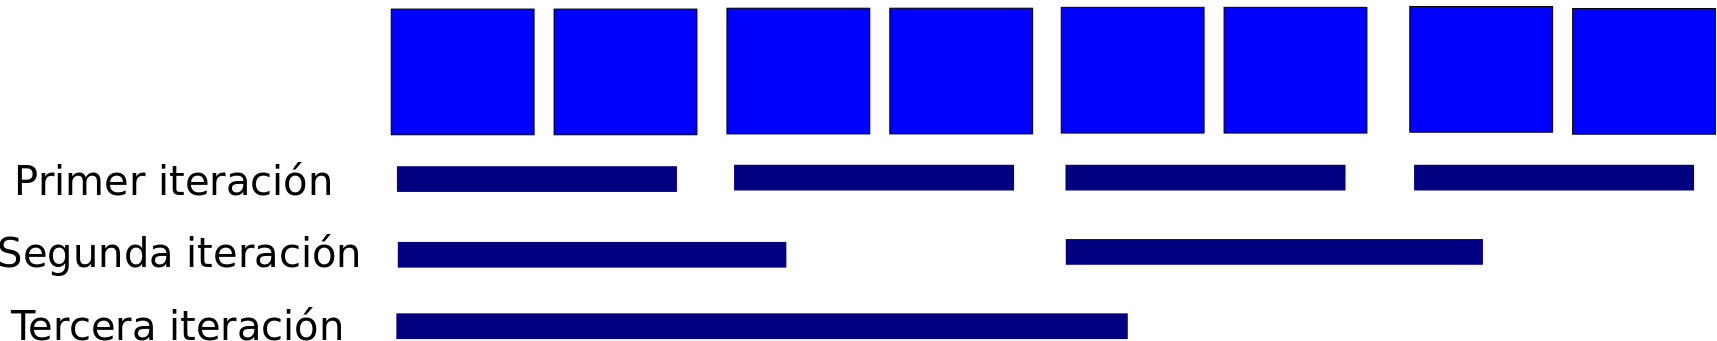
\includegraphics[width=\plotwidth]{images/reductions.png}
   \caption{Esquema de las reducciones realizadas en cada iteraci\'on del ciclo de la
   figura~\ref{code:sum-matrix-bench-code}.}
   \label{fig:sum-matrix-bench-reduce}
\end{figure}

Claramente este algoritmo debiera producir un mejor tiempo de ejecuci\'on, en
teor\'ia, utilizando m\'ultiples procesadores. Esto suena razonable considerando
que al menos algunas operaciones son delegadas a otros procesadores.

Medimos los tiempos de reducir $128$ matrices de $1024 \times 1024$ elementos de punto
flotante de precisi\'on simple, variando la cantidad de hilos de ejecuci\'on a
utilizar. Para compensar por primeras lecturas y otros factores, se tomo un promedio
de los resultados despu\'es de realizar 20 mediciones sucesivas con la misma
cantidad de \textit{threads}. Todo el c\'odigo se incluye en un ap\'endice de este
trabajo.

Como puede verse en la figura~\ref{fig:sum-matrix-bench-result}, los resultados
son desalentadores: el uso de multiprocesamiento no es \'util para este problema.

\begin{figure}[htbp]
   \centering
   \includegraphics[width=\plotwidth]{plots/cpu/scalability-matrix-sums.png}
   \caption{Tiempo en segundos para sumar 128 matrices de $1024 \times 1024$
   elementos, seg\'un la cantidad de threads usados. Los resultados corresponden
   a un promedio de 20 corridas, consecutivas para cada cantidad.}
   \label{fig:sum-matrix-bench-result}
\end{figure}

Observando el problema en si, notamos lo siguiente: Cada elemento de las
matrices a sumar es accedido de memoria una \'unica vez y el \'unico computo
realizado con este elemento es una suma con los dem\'as. La relaci\'on entre
lecturas de memoria y operaciones con los datos le\'idos es por lo tanto muy baja.

Observemos adem\'as que, al no utilizarse los datos m\'ultiples veces, cada l\'inea
de datos tiene un \textit{cache miss} asociado (el de la l\'inea donde reside) que
no se ve compensado por uso del mismo mientras reside en cach\'e.

Este tipo de problemas se denomina \textit{memory bound}, ya que la velocidad del
\textit{bus} de memoria y la organizaci\'on de la misma es el factor determinante,
no la capacidad de computo.

Esto implica que, pasado un cierto punto de velocidad de reloj de procesador y
cantidad de n\'ucleos, incrementar estos no produce mejoras apreciables. Esto es
lo que se puede ver en la figura~\ref{fig:sum-matrix-bench-result}.

Ver que ese es el caso en la prueba de concepto realizada requiere herramientas
de an\'alisis m\'as sofisticadas. En nuestro caso utilizamos la herramienta de
c\'odigo abierto \textit{perf}. Esta herramienta usa los contadores de
\textit{performance} que presentamos en las secciones anteriores, para dar estad\'isticas
a nivel arquitectural de la aplicaci\'on y de muy fino detalle, como por
ejemplo cantidad de \textit{cache misses}, \textit{stalls} en el pipeline,
cantidad de \textit{branch mispredictions}, etc.

%TODO(jpdarago): Agregar una introduccion a los contadores de perf

A continuaci\'on se muestran los resultados de correr
un an\'alisis de \textit{perf} para 1 y 12 hilos simult\'aneos en la m\'aquina de
prueba. De inter\'es es el valor de \texttt{stalled-cycles-frontend}. Este valor
corresponde al contador de \textit{performance} \texttt{UOPS\_ISSUED.ANY}. Este
contador registra los eventos en los que el procesador esta \textit{stalleado},
es decir el \textit{pipeline } no avanza pues esta a la espera de datos que
lleguen de memoria principal o un evento similar~\cite{Intel3B}. En este
caso, parece ser que este factor es un limitante extremadamente fuerte

{\footnotesize
\begin{verbatim}
$ perf stat -B ./benchmark 1024 128 1
1 0.180418953613844

 Performance counter stats for './benchmark 1024 128 1':

       2076,031257 task-clock                #    0,998 CPUs utilized
               225 context-switches          #    0,108 K/sec
                 0 cpu-migrations            #    0,000 K/sec
            67.583 page-faults               #    0,033 M/sec
     4.325.757.818 cycles                    #    2,084 GHz
     3.685.447.979 stalled-cycles-frontend   #   85,20% frontend cycles idle
   <not supported> stalled-cycles-backend
     1.801.562.845 instructions              #    0,42  insns per cycle
                                             #    2,05  stalled cycles per insn
       220.639.658 branches                  #  106,280 M/sec
           191.368 branch-misses             #    0,09% of all branches

       2,080571933 seconds time elapsed

$ perf stat -B ./benchmark 1024 128 12
12 0.182727314613294

 Performance counter stats for './benchmark 1024 128 12':

      22160,476291 task-clock                #   10,531 CPUs utilized
             2.402 context-switches          #    0,108 K/sec
                17 cpu-migrations            #    0,001 K/sec
            66.704 page-faults               #    0,003 M/sec
    46.310.011.626 cycles                    #    2,090 GHz
    42.797.073.792 stalled-cycles-frontend   #   92,41% frontend cycles idle
   <not supported> stalled-cycles-backend
     9.369.677.336 instructions              #    0,20  insns per cycle
                                             #    4,57  stalled cycles per insn
     2.657.329.767 branches                  #  119,913 M/sec
           687.016 branch-misses             #    0,03% of all branches

       2,104317579 seconds time elapsed
\end{verbatim}
}

Esto lleva a concluir que esta operaci\'on final impactar\'ia muy
negativamente en la escalabilidad de la implementaci\'on, y que por lo tanto a
medida que la cantidad de procesadores se incrementara esta secci\'on del
c\'odigo se har\'ia mucho m\'as pesada. Por lo tanto, se busc\'o reorganizar
este ciclo para no necesitar una matriz separada.

El ciclo a modificar esta en la figura~\ref{algo:rmm-output-previous}.
Se ve f\'acilmente que esto es posible si se invierten los ciclos internos y externos en
el algoritmo, para poder dividir los \'indices de la matriz global entre m\'ultiples
hilos de ejecuci\'on.

\begin{algorithm}[H]
    \centering
    \caption{C\'alculo original de la matriz de Kohn-Sham}
    \label{algo:rmm-output-previous}
    \begin{algorithmic}
        \State $R \gets 0_{m,n}$
        \State $F \gets functions(PG)$
        \ForAll{$p \in points(PG)$}
            \ForAll{$i,j \in m \times n$}
            \State $R_{i,j} \gets R_{i,j} + F_{p,i} \cdot F_{p,j} \cdot factors_{p}$
            \EndFor
        \EndFor
        \ForAll{$i,j \in fock\_indexes(PG)$}
            \State $KS_{i,j} \gets KS_{i,j} + R_{i,j}$
        \EndFor
    \end{algorithmic}
\end{algorithm}

La versi\'on modificada puede verse en la figura~\ref{algo:rmm-output-new}. Lo que
se hace para este caso es recorrer los \'indices a actualizar de la matriz total
y luego obtener la contribuci\'on de todos los puntos. Dado que cada \'indice debe
ser actualizado por, a lo sumo, un solo hilo de ejecuci\'on, no hay necesidad de
clonar matrices y reducirlas.

\begin{algorithm}[H]
    \centering
    \caption{C\'alculo de la matriz de Kohn-Sham reestructurado para paralelismo}
    \label{algo:rmm-output-new}
    \begin{algorithmic}
        \State $R \gets 0_{m,n}$
        \State $F \gets functions(PG)^T$
        \ForAll{$i,j \in indexes$}
            \State $KS_{i,j} \gets KS_{i,j} + \displaystyle \Sigma_{p \in points(PG)} F_{p,i} \cdot F_{p,j} \cdot factors_{p}$
        \EndFor
    \end{algorithmic}
\end{algorithm}

Un problema provocado por la implementaci\'on es que recorre la matriz de funciones
en orden de columnas, en lugar de orden por filas. Este orden es poco amigable
para los caches ya que cada fila de la matriz probablemente resida en l\'ineas de
cach\'e diferentes. Esto puede disminuir apreciablemente la performance del algoritmo.
Adem\'as, lastima su escalabilidad en procesadores, al incrementarse la cantidad de
invalidaciones de cach\'e y por lo tanto el \textit{overhead} del algoritmo de
coherencia entre caches intreprocesadores.

La soluci\'on a este problema es sin embargo sencilla, trasponiendo la matriz de
valores de funciones. La misma puede trasponerse una vez y almacenarse en memoria
RAM al iniciar las iteraciones, teniendo por lo tanto un relativo bajo costo de
creaci\'on, y el impacto que tiene en la cantidad de \textit{misses} de cach\'e.

Esta modificaci\'on del algoritmo introduce un nuevo aspecto a considerar, similar
a las consideraciones hechas para la cantidad de puntos y funciones: una poca
cantidad de \'indices a actualizar en un mismo grupo eclipsa el \textit{overhead}
que introduce el uso de OpenMP. La cantidad de \'indices de la matriz de Kohn-Sham a
actualizar tambi\'en tiene una distribuci\'on bastante dispar, como puede verse
para el caso de ejemplo de hemoglobina en la figura~\ref{fig:histogram-indexes-hemo}.

\begin{figure}[htbp]
   \centering
   \includegraphics[width=\plotwidth]{plots/cpu/histogram-indexes-hemo.png}
   \caption{Cantidad de \'indices a actualizar de la matriz de Kohn-Sham.}
   \label{fig:histogram-indexes-hemo}
\end{figure}

Esto enfatiza a\'un m\'as la necesidad de utilizar una paralelizaci\'on h\'ibrida
para grupos chicos y grandes, ya que ahora se tiene un factor m\'as que determina
cuanto trabajo se le asigna a los \textit{threads}.

Estos dos factores se tienen en cuenta en la funci\'on que determina si un grupo
es considerado grande o no. Para considerar un grupo grande, el mismo debe tener
una cantidad de puntos y una cantidad de \'indices en la matriz de Kohn-Sham mayor que
un valor de frontera (\textit{threshold}) multiplicado por la cantidad de hilos de
ejecuci\'on a realizar. Este valor es ajustable y mostraremos los resultados
correspondientes a tomar la mejor elecci\'on, siendo interesante su efecto en el
tiempo de ejecuci\'on de la iteraci\'on.

\subsection{Algoritmo de balanceo}

Por \'ultimo, si bien el algoritmo de particionado y la funci\'on de costo son
buenas para los casos estudiados, no son perfectas. Como puede verse en la
figura~\ref{fig:lio-imbalance-between-loads}, hay una diferencia entre cargas
no despreciable en algunos casos, con lo cual todav\'ia se puede obtener algo de
mejoras en \textit{performance} entre iteraciones utilizando balanceo de cargas,
que obtuvo buenos resultados en la implementaci\'on para GPGPUS.

\begin{figure}[htbp]
   \centering
   \includegraphics[width=\plotwidth]{plots/cpu/group-split-differences.png}
   \caption{Comparaci\'on de los tiempos de ejecuci\'on para las distintas
   cargas asignadas a cada hilo de ejecuci\'on en el caso de la hemoglobina.}
   \label{fig:lio-imbalance-between-loads}
\end{figure}

El algoritmo es muy similar, se mide el tiempo de \textit{runtime} para cada
grupo de cada carga, y cuanto dura cada una de ellas. Luego, se repite una
cantidad de veces (5 veces, como la implementaci\'on de balanceo en multiplaca)
que se mueve una cierta cantidad de grupos desde la carga m\'as pesada a la
m\'as liviana, de manera de no pasarse de la diferencia temporal que hay entre
ellas. Una vez movidos los grupos correspondientes, y tal que la diferencia
entre los dos estimativos es menor que el 5\% del peso total de la carga m\'as
pesada, se prosigue por encontrar las otras dos cargas m\'as dispares y
rebalancearlas. Para m\'as detalles del algoritmo puede verse la secci\'on
de balanceo de cargas de la implementaci\'on en GPU.

El costo computacional ya se vi\'o anteriormente que resulta bajo. En el caso
de la hemoglobina se consigue menos del 5\% de diferencia en una iteraci\'on
de rebalanceo, obteniendose los resultados de la figura~\ref{fig:lio-imbalance-fixed}.

\begin{figure}[htbp]
   \centering
   \includegraphics[width=\plotwidth]{plots/cpu/group-split-differences-post-balance.png}
   \caption{Comparaci\'on de los tiempos de ejecuci\'on para las distintas
   cargas asignadas a cada hilo de ejecuci\'on en el caso de la hemoglobina,
   luego de rebalancear}
   \label{fig:lio-imbalance-fixed}
\end{figure}



